\documentclass[10pt,letterpaper]{book}
%\usepackage[a5paper]{geometry}%if printed as book
%\usepackage[papersize={6in,9in},right=.5in,left=.5in,top=.75in,bottom=.5in,bindingoffset=.375in,heightrounded]{geometry}
\usepackage[paper=letterpaper,layoutsize={6in,9in},bindingoffset=.375in, heightrounded, showframe, showcrop]{geometry}%default geometry pretty close to golden ratio, guttenburg Tschichold's "golden canon of page construction"
%\usepackage[papersize={6in,9in},layoutsize={6in,9in},bindingoffset=.375in, heightrounded]{geometry}%this is for printing

%\usepackage{layout}
\usepackage[utf8]{inputenc}
\usepackage{amsmath}
\allowdisplaybreaks[4]
\usepackage{amsfonts}
\usepackage{amssymb}
\usepackage[american,cuteinductors]{circuitikz}
\usepackage{hyperref}
\usepackage{tabularx}
\usepackage{booktabs}

\usepackage{listings}

\author{Scott Howard scott@scimpy.com}
\title{Scimpy:\\ \textbf{S}ound \textbf{C}ard based \textbf{I}mpedance \textbf{M}easurements in \textbf{Py}thon}
\date{Last Revision: \today}
\begin{document}
\frontmatter

%\layout
\maketitle

\section*{Copyright}
test

\section*{License}
test


\tableofcontents

\mainmatter
\part{Using Scimpy}
\chapter{Introduction}
``Hence the expression Butterworth box. However, in the spite of the phonetic similarity, butter boxes are not in general suitable as loudspeaker enclosures." -- A. N. Thiele
\chapter{Usage}
test
\section{How to Connect Hardware}
Headphones are typically 32 ohms, so want to use 20 ohm resistor to protect circuits?

line out? does it have enough current?

line in: 600-47 kOhms (low impedance)
microphone, more sensitive but powered (need AC coupling?)
\section{How to Use the Software}
\subsection{Taking Data}
\subsection{Interpreting Data}
\part{Theory}
\chapter{Impedance}\label{Impedance}
\textbf{Modern amps have lots of current, digital feedback - is impedance important? probably not, except to help cross over maybe... Impedance measurements can get you info on internal parameters, help tune/design box for example!}

Speaker impedance represents how much voltage will be needed to drive 1~A of current  through the speaker voice coil. Higher resistance means that speaker response will drop, as it is harder to push current through it. Due to electrical, mechanical, and acoustical effects, impedance changes with frequency -- thus changing how the speaker sounds. If speaker impedance drops too low, more current will be needed from the amplifier. Over-driving the speaker amplifier risks distortion and overheating the amplifier. Additionally, passive cross-over circuits (i.e., what splits the signal to tweeter and woofer) are designed to work with loads whose impedance do not change with frequency; poor impedance matching reduces cross-over performance

An ``impedance matching" circuit can correct this poor performance. The circuit is designed such that the combined impedance of the speaker and circuit us the same for all frequencies, and thus avoiding signal distortion and amplifier damage.

Impedance circuits can be classified as active or passive. Active circuits are easier to design but are expensive and require additional power. Passive circuits are cheaper, but a well designed circuit will perform as well as an active system. However, designing such circuits requires specialized equipment and software. Thus the motivation for this project: develop a widely available, easy-to-use tool to measure impedance and provide impedance matching circuit designs.

Section \ref{Impedance} will describe how to measure impedance. Section \ref{loudspeakers} will then build a model of loudspeaker performance.
\section{Electrical Impedance}
Voltage ($V$) and current ($I$) are related to each other through the following expressions describing resistors (with resistance $R$), capacitors (with capacitance $C$), and inductors (with inductance, $L$):
\begin{align}\label{electrical_eqs}
V&=IR & V&=L\frac{\partial I}{\partial t} & I=C\frac{\partial V}{\partial t}
\end{align}

To understand their frequency response, we use generic time harmonic signals:
\begin{align}\label{timeharmonic}
V=V_0\cos(\omega t + \phi_{_V})&=\Re{ \left\{ \hat{V}e^{i\omega t}\right\} }\\
I=I_0\cos(\omega t + \phi_{_I})&=\Re{ \left\{ \hat{I}e^{i\omega t}\right\} }
\end{align}

Where $\hat{V}(\omega)=V_0(\omega)e^{i\phi_{_V}(\omega)}$ and $\hat{I}(\omega)=I_0(\omega)e^{i\phi_{_I}(\omega)}$ are the phasor representation of voltage and current. Combining Equations~\ref{electrical_eqs} and \ref{timeharmonic} we can see that the phasor voltage and currents are proportional to each other by a factor of $Z$ for each of the circuit elements.
\begin{align}
\frac{\hat{V}}{\hat{I}}&=Z_R=R & Z_L&=i\omega L & Z_C&=\frac{1}{i\omega C}
\end{align}

Phasors allows us to easily calculate the relationship between voltage and current in complex circuits. For example, Figure~\ref{circuit1} can be represented using phasor sources and complex impedances as in Figure~\ref{circuit2}.

\begin{figure}
\centering
\begin{circuitikz}
  \draw (0,0)
  to[V=$V_0\cos(\omega t)$] (0,2) % The voltage source
  to[short] (1,2)
  to[short] (2,2)
  to[R=$R$] (2,0) % The resistor
  to[short] (0,0);
  \draw (2,2)
  to[short] (4,2)
  to[L=$L$] (4,0)
  to[short] (2,0);
  \draw (4,2)
  to[short] (6,2)
  to[C=$C$] (6,0)
  to[short] (4,0);
\end{circuitikz}
\caption{Example circuit}\label{circuit1}
\end{figure}

\begin{figure}
\centering
\begin{circuitikz}
  \draw (0,0)
  to[V=\mbox{$\hat{V}=V_0e^{i\omega t}$}] (0,2) % The voltage source
  to[short] (1,2)
  to[short] (2,2)
  to[generic=\mbox{$Z_R$}] (2,0) % The resistor
  to[short] (0,0);
  \draw (2,2)
  to[short] (4,2)
  to[generic=\mbox{$Z_L$}] (4,0)
  to[short] (2,0);
  \draw (4,2)
  to[short] (6,2)
  to[generic=\mbox{$Z_C$}] (6,0)
  to[short] (4,0);
\end{circuitikz}
\caption{Example circuit with complex impedances}\label{circuit2}
\end{figure}

Using standard circuit analysis, you can calculate the current coming out of the voltage source by treating each circuit element as if it was a resistor.
\begin{align}
Z=\left(\frac{1}{Z_R}+\frac{1}{Z_C}+\frac{1}{Z_L}\right)^{-1}
\end{align}
\begin{align}
\hat{I}&=\hat{V}\left(\frac{Z_CZ_L+Z_RZ_L+Z_RZ_C}{Z_R+Z_C+Z_L}\right)\\
&=V_0e^{i\omega t}\left( \frac{L/C+i\left[ -R/(\omega C)+\omega RL\right]}{R+i\left(\omega L - \omega/C\right)} \right)\label{complex_imp}
\end{align}

Current, $I$, can now be found by taking the real part of $\hat{I}$.

\section{Impedance Matching}
Our challenge is to design a circuit that makes the impedance constant for all frequencies. For example, a speaker has an impedance $Z=R+Z_0$, which represents a DC ($\omega=0$) resistance of $R$ and a frequency dependant impedance $Z_0$. to match impedance, a circuit with impedance $Z_1$ is added in parallel to the speaker, as depicted in Figure~\ref{simplespeaker}. The equivalent impedance is $Z=\frac{Z_1(R+Z_0)}{Z_1+Z_0+R}$. Setting $Z=R$ and solving for $Z_1$ yields:
\begin{align}\label{impmatching}
Z_1=R+\frac{R^2}{Z_0}
\end{align}

Equation \ref{impmatching} represents how we will design our impedance matching circuit. The circuit will consist of a resistor of resistance $R$ in series with a circuit that is the ``electric dual" of $Z_0$ scaled by $R^2$. The electric dual of a circuit with impedance $Z$ is defined as the circuit with impedance $Z'=1/Z$.

\begin{enumerate}
\item Develop a circuit model for $Z_0$ (and thus the dual circuit model for $Z'_0$)
\item Measure $R+Z_0$ as a function of frequency to extract $R$ and the values of the elements in the circuit model.
\end{enumerate}

\begin{figure}
\centering
\begin{circuitikz}[yscale=0.75]
  \draw (0,0)
  to[open,o-o] (0,4) % The voltage source
  to[short] (2,4)
  to[generic=\mbox{$\hat{Z}_1$}] (2,0) % The resistor
  to[short] (0,0);
  \draw (2,4)
  to[short] (4,4)
  to[R=$R$] (4,2)
  to[generic=\mbox{$\hat{Z}_0$}] (4,0)
  to[short] (2,0);
\end{circuitikz}
\caption{Speaker impedance matching}\label{simplespeaker}
\end{figure}

\subsection{Why Impedance Matching Doesn't Matter Any More}
Impedance matching is important (1) to ensure that the amplifier doesn't overwork itself and (2) to ensure that cross-over circuits are properly tuned.

\textbf{Amplifiers in Overdrive:} Amplifiers can be modelled as voltage sources with some ``output impedance" representing the resistance the amplified signal sees leaving the amplifier. This is depicted in Figure \ref{fig:amp-out-imp} where $R_g$ is the output impedance of the amplifier, $v_L$ is the voltage across the load, and $\hat{Z}_L$ is the complex impedance of the load. The voltage seen by the speaker and the current delivered by the amp is:
\begin{align}
\hat{v}_L&=\hat{v}_0\frac{\hat{Z}_L}{R_g+\hat{Z}_L} & \hat{i}_L=\frac{\hat{v}_L}{\hat{Z}_L}=\frac{\hat{v}_0}{R_g+\hat{Z}_L}
\end{align}
which illustrates two potential problems. (1) If $R_g > \hat{Z}_L$, then the voltage  seen by the load (and thus audio response) will change with frequency since $\hat{Z}_L$ is a function of frequency. (2) If $\Re\{\hat{Z}_L\}$ becomes low at a specific frequency, $\hat{i}_L$ will increase rapidly with the risk of ``burning out" the amplifier as all the amplifier power is dissipated solely in the amplifier internal load.

\begin{figure}
\centering
\begin{circuitikz}
  \draw (0,0)
  to[V=$v_0$] (0,2) % The voltage source
  to[R=$R_g$] (2,2)
  to[generic=\mbox{$\hat{Z}_L$},v=$v_L$, i=$i_L$,o-o] (2,0)
  to[short] (0,0);
\end{circuitikz}
\caption{Amplifier Output Impedance}\label{fig:amp-out-imp}
\end{figure}

Originally, valve amplifiers (tube amps) were commonly used to amplify the small signal from audio sources, and exhibited $R_g$ of $100$s of $\Omega$ or more. As such it was important that $\hat{Z}_L$ remain real constant over all frequencies so that the tube does not burn out and performance remain consistent over all frequencies. Impedance matching achieved those goals. However, modern solid-state transistor-based amplifiers have near zero output impedance and therefore deliver the needed $\hat{v}_L$ without impedance matching. In essence, low $R_g$ allows solid-state amplifiers to output large $\hat{i}_L$ in order to maintain $v_L=v_0$.

\textbf{Impedance and Cross-Over Design:} Impedance matching also helps cross-over design, as a flat and real load is assumed. However, if the cross-over frequency is chosen to be away from any resonance (such as choosing a cross-over frequency of an octave larger than the speaker resonance $2\times f_s$), then impedance matching becomes less important as the load is essentially flat over the pass-band.

\subsection{Why Impedance Matching Still Matters}
Valve/tube amplifiers are popular among some audiophiles because they deliver a ``warmth" unlike solid-state amps. Usage in audio circuits requires impedance matching. That said, some commercial tube amplifier systems know modern speakers are not commonly impedance matched. That's why you see amplifiers using tube amplifiers as pre-amplifiers and solid-state amplifiers as buffers to drive speakers as an attempt to get the best of both worlds.

A well matched circuit ensures that maximum power is delivered to the load across all frequencies. Using impedance matching means the amplifier will not have to ``work as hard," and thus improve efficiency. If your amplifier is operating near the maximum output rating, it could be good to impedance match the system to ensure expected performance. However, it might be cheaper and easier to buy a bigger amplifier!

\subsection{Why Impedance \textit{Measurements} Still Matter}
so you know speaker specs to design cab

\section{Measuring Impedance}
Impedance testing is actually relatively straight forward. A function generator creates voltage to a circuit that has a resistor (of accurately known resistance $R_{test}$) in series with the speaker. The function generator creates a sinusoidal voltage with constant amplitude $V_0$ at different frequencies $\omega$. A volt meter measures the voltage across the test resistor, $v_r$, as a function of frequency $\omega$. The generic test system is described in Figure~\ref{imp_measure}. Speaker impedance can be found with the Equation~\ref{generic_imp}, below:
\begin{align}\label{generic_imp}
\hat{v}_s=\frac{ \hat{Z}_s V_0 }{ R_{test} + \hat{Z}_s } && \hat{i}_s=\hat{i}_r=\frac{\hat{v}_r}{R_{test}} && \hat{Z}_s=\frac{\hat{v}_s}{\hat{i}_s}=R_{test}\left( \frac{V_0}{\hat{v}_r} -1 \right)
\end{align}
All variables with carrots indicate complex numbers with a phase relative to the source, $V_0$.

Equation \ref{generic_imp} assumes the magnitude and phase of  $\hat{v}_1$ can be measured relative to the phase of the source with, for example, an oscilloscope locked in to the frequency and phase of the voltage source. If you don't have such a lock-in detection scheme (which few do), but do have time sensitive measurements (e.g., a sound card like we use in this project). You can rearrange Equation \ref{generic_imp} to be:
\begin{align}\label{generic_imp_2measure}
\hat{Z}_s=R_{test}\left( \frac{V_0 - \hat{v}_r}{\hat{v}_r}\right)=R_{test}\left( \frac{\hat{v}_s}{\hat{v}_r}\right)
\end{align}
which shows we need a another voltage meter to get $\hat{v}_s$. This is shown in Figure~\ref{imp_measure2}, and is the ciruit this project uses to find $\hat{Z}_s$ in Equation~\ref{generic_imp_2measure}).



Commonly, time sensitive measurements are impractical as hobbyist typically only have multimeters, which can measure AC RMS. If only the RMS magnitude of AC voltage can be measured, then the magnitude of $Z$ can be found as in Equation~\ref{generic_imp_mag}.
\begin{align}\label{generic_imp_mag}
\hat{\left|Z_s\right|}=\frac{\left| v_s \right| R_{test}}{\left| v_r \right|}
\end{align}

Note: Equation \ref{generic_imp_mag} differs from some hobbyist impedance measurement techniques\footnote{Sometimes incorrectly given as: $\left| Z_s \right| = R\left(\frac{ \left| V_0 \right|}{\left| v_r \right|}-1\right) $} which ignores the fact that phases of each of the voltages are not the same!

\begin{figure}
\centering
\begin{circuitikz}
  \draw (0,0)
  to[V=\mbox{$V_0\cos(\omega t)$}] (0,2) % The voltage source
  to[short] (1,2)
  to[R=$R_{test}$,i=$\hat{i}_r$,v=$\hat{v}_r$,o-o] (3,2) % The resistor
  to[short] (4,2)
  to[generic=\mbox{$\hat{Z}_s$},v=$\hat{v}_s$,i=$i_s$] (4,0)
  to[short] (0,0);
  \draw (1,2)
  to[short] (1,1)
  to[voltmeter] (3,1)
  to[short] (3,2);
\end{circuitikz}
\caption{Typically described speaker impedance measurement (requires voltmeter to be locked-in to the source phase)}\label{imp_measure}
\end{figure}

\begin{figure}
\centering
\begin{circuitikz}
  \draw (0,0)
  to[V=\mbox{$V_0\cos(\omega t)$}] (0,2) % The voltage source
  to[short] (1,2)
  to[R=$R_{test}$,i=$\hat{i}_r$,v=$\hat{v}_r$,o-o] (3,2) % The resistor
  to[short] (4,2)
  to[generic=\mbox{$\hat{Z}_s$},v=$\hat{v}_s$,i=$i_s$] (4,0)
  to[short] (0,0);
  \draw (1,2)
  to[short] (1,1)
  to[voltmeter] (3,1)
  to[short] (3,2);
  \draw (4,2)
  to[short,o-] (5.5,2)
  to[voltmeter, mirror] (5.5,0)
  to[short,-o] (4,0);
\end{circuitikz}
\caption{Speaker impedance matching (this project, no lock-in required)}\label{imp_measure2}
\end{figure}


Once $\hat{Z}$ or $\left| \hat{Z} \right|$ is found for different frequencies $\omega$, you can fit the data to the models in Section~\ref{loudspeakers} to extract the values needed to make the impedance matching circuit.

\section{Crossover Circuits and Impedance}

Scott notes:
Editorial Note About Directivity, Crossover Points \& Driver Selection by Dr. Floyd Toole

A good sounding loudspeaker needs to have smooth and flat on-axis frequency response and similar performance as we move far off axis.  We describe this in terms of directivity as a function of frequency, and although absolutely constant directivity is not necessary, smooth and gradually-changing directivity is a good objective.  In deciding on the drivers to be used in a speaker system it is necessary to ensure that at crossover frequencies the drivers have closely matching directivities.  This means that when the acoustic transition is made between, say, a woofer and a midrange, or a midrange and a tweeter, there is continuity in the directional sound radiation pattern. It is not sufficient just to have a good looking on-axis response.  So, in addition to selecting drivers for their useable bandwidths and power handling capabilities, we need to pay attention to their directional radiation patterns. The most difficult transitions occur when the transducers involved are very different in size.
Editorial Note by Steve Feinstein on Crossover Frequency Selection

A basic, ages-old but still true, rule of thumb states that a designer is usually safe when he crosses a driver over at double its resonant frequency. If a tweeter has an Fs of 1500 Hz, use a 3000 Hz crossover, minimum. If a midrange is 300 Hz, use 600 Hz.

Another good rule of thumb says, “18 dB down at resonance.” If a tweeter’s resonance is 1500 Hz, the voltage curve of the crossover should show the tweeter section being down 18 dB from “0 dB.” That kind of conservatism all but assures no tweeter burn-out.

This was the “rule” at a major speaker company I used to work at, and the engineers all hated it, because it was so conservative and resulted in very high tweeter crossover points. But we almost never lost a tweeter and our warranty costs were vanishingly low. ‘Real world’ vs. ‘theory.’
from:
http://www.audioholics.com/loudspeaker-design/crossovers



START HERE:

Cross-over circuits are needed to separate the sound signal into high and low frequency components. Ideally for dipole speakers, you want a ``switch" that sends low frequency below some cross-over frequency $\omega_c$ only to the woofer and higher frequencies only to the tweeter. Practically, some leakage will occur in separating the signals such that some low frequencies will end up at the tweeter, and high at the woofer.  These negative effects define the engineering problem.

Cross-over circuits are either classified as active (powered) or passive (unpowered). \textit{Active cross-overs} use operational amplifiers (op amps) that can drive loads with complex $\hat{Z}$ uniformly across all frequencies and thus do not need impedance matching circuits. However, they tend to be a bit complicated, expensive, and require additional power. \textit{Passive cross-overs} are cheaper, simpler, and don't require extra power -- but do require extra care in design to achieve the same same theoretical performance as active cross-overs. Since we have the tools to properly design cross-overs, we will consider passive cross-overs.

After building the impedance matching circuit, we need to build a circuit that separates the low and high frequency components. Next, the simplest electric filter is an inductor or a capacitor in series with a resistor to make a low-pass and high-pass filter, respectively, as in Figure~\ref{filters}.

\begin{figure}
\centering
\begin{circuitikz}
  \draw (0,0)
  to[open,v^>=$v_i$,o-o] (0,2) % The voltage source
  to[short] (1,2)
  to[generic=$\hat{Z}$] (3,2) % The resistor
  to[short] (4,2)
  to[R=$R_S$,v=$\hat{v}_o$,o-o] (4,0)
  to[short] (0,0);
\end{circuitikz}
\caption{First order filter}\label{filters}
\end{figure}

The transfer function ($\hat{H}$, the ratio of output to input voltage) can be found for $\hat{Z}=i\omega L$ and $\hat{Z}=\frac{1}{i\omega C}$
\begin{align}
\hat{H}_{LP}(\omega)=\left( {1+\frac{i\omega L}{R}} \right)^{-1}
&=\left( {1+\frac{\omega^2}{ \omega_c^2}}\right)^{-\frac{1}{2}} e^{\tan^{-1}\left( \frac{\omega}{\omega_c}\right)}\\
\hat{H}_{HP}(\omega)
=\left( {1+\frac{1}{i \omega R C}} \right)^{-1}
&=\left( {1+\frac{\omega_c^2}{\omega^2 }}\right)^{-\frac{1}{2}} e^{\tan^{-1}\left( \frac{\omega_c}{\omega}\right)}
\end{align}

$L$ and $C$ are picked for a given cross-over frequency such that $L=\frac{R}{\omega_c}$ and $C=\frac{1}{R\omega_c}$. Note that the sum of both speaker outputs $\hat{H}_{LP}(\omega)+\hat{H}_{HP}(\omega)~=~1$ for all frequencies! That means that the signal is transferred perfectly in amplitude (volume) and phase (audible delay) at every frequency. However, each driver demonstrates a group phase delay ($\partial \phi / \partial \omega$) in the pass-bands, so how can it appear to have zero-phase? Well, it's a bit of a trick in that the system ``uses"  \textit{both} speakers to correct for this variable delay as a function of frequency. Low frequencies coming from the woofer have small delay (phase), while those low frequencies in the tweeter have a lot of delay. As frequency increases, woofer delay increases and tweeter delay decreases. The apparent phase (delay) is unchanged. This is not ideal as it relies on driving your tweeter lower than designed (risking overheating and damage) and your woofer higher than intended (excited standing waves/nodes within the woofer driver which degrades sound quality). Therefore, high-order filters are preferred.

High order filters (i.e., ones that separate tweeter and woofer signals better) can be used, but requires more parts. See, for example, Linkwitz-Riley (LR) filters for a high-order filter. The LR2 filter design is shown in Figure~\ref{LRfilters}. Choosing $Z_1=Z_2$ and $R_s=R_1$, you can calculate transfer functions in the Maxima computer algebra system (left for the reader):
% put this in and plot?!
%\begin{verbatim}
%ZL1:%i*w*L1;
%Zsub:((R1+ZL1)^(-1)+1/R1)^(-1);
%transferfunc:Zsub/(Zsub+ZL1);
%(declare(w,mainvar),ratexpand(transferfunc));
%\end{verbatim}

You can see that the LR2 filter has many positive features compared to our simple filter (1) Faster roll-off (12 dB/octave versus 6 dB/octave) -- better separation of frequencies to protect the drivers. (2) Phase is flat (low group delay) in the pass-bands. There is, however, some group delay around cross-over. (3) Constant phase offset between woofer \& tweeter for all frequencies. Offset is 180$^\circ$, so you need to to wire one of the drivers backwards (negative polarity). (4) Like our simple system, choose $L=R/\omega_c$ and $C=1/(\omega_c R)$.



\begin{figure}
\centering
\begin{circuitikz}
  \draw (0,0)
  to[open,v^>=$v_i$,o-o] (0,2) % The voltage source
  to[short] (1,2)
  to[generic=$\hat{Z_1}$] (3,2) % The resistor
  to[R=$R_1$,] (3,0)
  to[short] (0,0);
  \draw (3,2)
  to[generic=$\hat{Z_2}$] (5,2)
  to[R=$R_S$,v=$\hat{v}_o$,o-o] (5,0)
  to[short] (3,0);  
\end{circuitikz}
\caption{Linkwitz-Riley Second Order Filter (LR2)}\label{LRfilters}
\end{figure}




%\section{Correct for difference in efficiency L-pad}

\chapter{How Do Loudspeakers Work?}\label{loudspeakers}
This section describes and summarizes a common mathematical model for aiding loudspeaker design. This approach was developed by the pioneers Neville Thiele of the Australian Broadcasting Commission, and Richard H. Small of the University of Sydney, and the parameters are commonly known as the ``Thiele/Small Parameters."

A loudspeaker converts electrical signals to sound waves by using the signal electrical voltage to drive a current which applies a force on a speaker membrane that in turn pushes a volume air. This pushed volume of air propagates as a sound wave to the listener.

To understand this process, we will break down the electrical, mechanical, and acoustical systems individually. We will also describe how each are connected. From the individual system models and our understanding of how they are connected, we will finally integrate them in to a complete single model which can be used to describe how loudspeakers work.
\section{Electrical Model}
A loudspeaker driver is fundamentally a system that translates electrical current to air motion. Current through a coil of wires (called the voice coil) interacts with a permanent magnet, as described in Figure~\ref{speaker_diagram}\footnote{By Iain, png by Rohitbd [CC-BY-SA-3.0], via Wikimedia Commons}. Wire, itself, is a resistor; when coiled a wire a an inductor; and the time varying magnetic field created by and inductor induces ``eddy currents" in nearby conductors which act as a resistor in parallel with the inductor. This electrical current is then can be coupled to the mechanical vibrations (discussed in Section~\ref{mechanical_section}). The electrical model is thus described in Figure~\ref{electrical_model}. Where $R_{vc}$ is the DC resistance of the voice coil, $L_{vc}$ is the inductance of the voice coil, $\hat{Z}_e$ is the electrical impedance equivalent to the mechanical impedance due to the electrical-mechanical coupling, and $R_{eddy}$ is the effective resistance due to eddy currents which is typically very high and frequently ignored in models. Finally, the current $i_e$ is the current that couples to mechanical motion described by $\hat{Z}_e$ as described in Section~\ref{mechanical_section}.

\begin{figure}
\centering
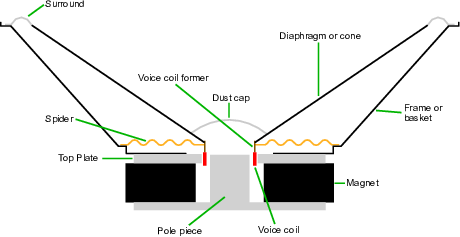
\includegraphics[width=0.75\textwidth]{Speaker-cross-section.png}
\caption[Loudspeaker Driver]{Loudspeaker Driver}
\label{speaker_diagram}
\end{figure}

\begin{figure}
\centering
\begin{circuitikz}
  \draw (0,0)
  to[open,v^>=$v_i$,o-o] (0,2) % The voltage source
  to[R=$R_e$] (2,2) % The resistor
  to[L=$L_e$,mirror] (4,2)
  to[short] (5,2)
  to[generic=$\hat{Z_e}$,i=$i_e$] (5,0)
  to[short] (0,0);
  \draw (2,2)
  to[short] (2,3)
  to[R=$R_{eddy}$] (4,3)
  to[short] (4,2);
\end{circuitikz}
\caption{Electrical Model}\label{electrical_model}
\end{figure}


\section{Mechanical Model}\label{mechanical_section}
Electric current is coupled to mechanical motion by the Loretnz Force equation:
\begin{align}
\mathbf{F}=Q\mathbf{E}+Q\mathbf{v}\times \mathbf{B}=Q\mathbf{E}+Q\ell\mathbf{I}\times \mathbf{B}
\end{align}
Where $F$ is force, $Q$ is charge, $v$ is velocity of the charge, and $B$ is the magnetic field (i.e., the length of the coil), $\ell$ is length of the wire in the field, and $I$ is the current. When current is moving in the wire, it exerts a force of
\begin{align}
F=IB\ell\label{force_current}
\end{align}
When a wire moves perpendicular to a magnetic field, carriers inside the wire feel a force of $F_B=QvB$. This force pushes electrons to one end of the wire, which creates a Coulomb force of $F_E=QE$. These two forces sum to zero, so $vB=-E$. This allows us to connect voltage across the coil, $V$, to velocity, $v$:
\begin{align}
V=-\int E\,d\ell=\int vB\,d\ell=vB\ell\label{velocity_potential}
\end{align}
From Equations \ref{force_current} and \ref{velocity_potential}, electrical impedance can be found in terms of force $F$ and $v$ in a mechanical system:
\begin{align}
\hat{Z}_e=\frac{V}{I}=\frac{v}{F}\left(B\ell\right)^2
\end{align}

To continue with our model, we need to find the relationship between $v$ and $F$, so we turn to Newton's law of motion and Hook's law for a dampened mass on a spring:
\begin{align}
\sum F&=M_{ms}\frac{d^2x}{dt^2}\\
F-\frac{1}{C_{ms}}x&=M_{ms}\frac{d^2x}{dt^2}+R_{ms}\frac{dx}{dt}\\
F&=M_{ms}\frac{dv}{dt}+R_{ms}v+\frac{1}{C_{ms}}\int v\,dt\\
F(\omega)&=i\omega M_{ms}v+R_{ms}v+\frac{1}{i\omega C_{ms}}v\label{force_equation}
\end{align}
where $M_{ms}$ is the mass of the diaphragm and coil (and acoustic mass), $C_{ms}$ is the compliance of the suspension (i.e., $1/k$ of Hooke's Law), and $R_{ms}$ represents the coefficient of friction (mechanical resistance to motion). From Equation~\ref{force_equation}, you can see that we can actually model mechanical systems as electrical circuits. In such a circuit,  voltages represent force, current represents velocity, inductance is mass, electrical resistance is mechanical resistance, and capacitance is compliance. Mechanical impedance, is thus:
\begin{align}
\hat{Z}_m&=\frac{F}{v}& \hat{Z}_e &= \hat{Z}_m^{-1} (B\ell)^2\label{mech_imp_dual}
\end{align}
Equation~\ref{mech_imp_dual} shows that if we represent our mechanical system as a mechanical circuit and find the mechanical impedance, the equivalent electric circuit is the dual of the mechanical circuit scaled by $(B\ell)^2$.

The mechanical system in Equation~\ref{force_equation} describes the speaker in vacuum, that is without interacting with air. The driver will push a volume of air to generate sound, and thus is an additional complex component in our circuit. Therefore the complete mechanical circuit is described in Figure~\ref{mechanical_model}.
\begin{figure}
\centering
\begin{circuitikz}
  \draw (0,0)
  to[open,v^>=$F$,o-o] (0,2) % The voltage source
  to[L=$M_{md}$] (2,2) % The resistor
  to[R=$R_{ms}$] (4,2)
  to[C=$C_{ms}$] (6,2)
  to[generic=$\hat{Z_m}$,i=$v$] (6,0)
  to[short] (0,0);
\end{circuitikz}
\caption{Mechanical Model}\label{mechanical_model}
\end{figure}



\section{Acoustical Model}\label{sec:acoustic_model}
From Section~\ref{mechanical_section}, we found a way to find the velocity the diaphragm will move as a function of input current. The moving diaphragm will push air and create a pressure wave, which is what we will hear. The speaker diaphragm pushes the following $V$ of air per second:
\begin{align}
Q=S_dv\label{eq:volume_velocity}
\end{align}
Where $Q$ is the volume velocity, $v$ is diaphragm velocity as found in Section~\ref{mechanical_section}, and $S_d$ is the area of the driver diaphragm. Also, it is possible to convert between mechanical and acoustic impedances by using the speaker diaphragm area $S_d$:
\begin{align}
Z_m=\frac{F}{v}=\frac{pS_d}{Q/S_d}= S_d^2 Z_a\label{eq:acoustic-to-mech_imp}
\end{align}

When mounted in a speaker enclosure, the air pushed/pulled from the front of the diaphragm radiates as sound waves while the air pushed/pulled from the back of the driver is shielded from the listener. This is because the sound waves from the back are perfectly out of phase from the front, and thus will lead to audio nulls in the room.

To stop this interference, the air pushed/pulled from the back of the driver is typically enclosed in a box. Through some acoustic tricks, one can invert the phase of the rear acoustic waves by the use of a ``port" or "bass reflex" which is essentially a tube opening up to the space the inside of the speaker enclosure. See Figure~\ref{bass_reflex}~\footnote{By Rohitbd, original by Melancholie.\\
CC-BY-SA 3.0, https://en.wikipedia.org/w/index.php?curid=2745689}.

\begin{figure}
\centering
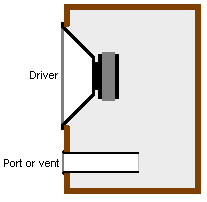
\includegraphics[height=0.25\textheight]{Bass_reflex_spk.png}
\caption{Bass Reflex Speaker or Vented Speaker Enclosure}\label{bass_reflex}
\end{figure}

We will consider this vented enclosure as our model since it is an extremely common enclosure  and the model can be easily adapted for other enclosures. First, we must find what the change in pressure $p$ is caused by $Q$. We know that pressure is increased per percent change in gas volume in the box $V_B$ by a factor of compressibility$^{-1}=\rho c^2$ :
\begin{align}
p&=\rho c^2 \frac{\Delta V_B}{V_B}=\rho c^2 \frac{\int Q_B dt}{V_B}\\
\hat{p}&=\frac{\rho c^2}{i\omega V_B}\hat{Q}_B=\frac{1}{i\omega C_{ab}}\hat{Q}_B\label{acoustic_compression}
\end{align}
where $Q_B$ is the volume velocity in to the box, $\rho$ is gas density, $c$ is the speed of sound, and $C_{ab}=\frac{V_B}{\rho c^2}$ is the acoustic capacitance of the box.

This increase of pressure inside the box will cause air flow in 
the port or vent, and acoustic radiation away from the vent. This air flow in a vent with area $A_v$, length $\ell_v$, volume $V_v$ will cause a pressure drop due to Newton's Law:
\begin{align}
F&=m\frac{dv}{dt}+\frac{\mu V_v}{\kappa} v\\
p&=\rho \frac{\ell_v}{A_v}\frac{dQ_v}{dt}+\frac{\mu \ell_v}{\kappa A} v\\
\hat{p}&=i\omega\rho \frac{\ell_v}{A_v}\hat{Q}_v+\frac{\mu \ell_v}{\kappa A_v} \hat{Q}_v\\
\hat{p}&=i\omega L_{av} \hat{Q}_v+R_{av} \hat{Q}_v \label{acoustic_flow}
\end{align}
where the second term is Darcy's law that describes $Q$ in a porous medium \textit{permeability} of $\kappa$ and viscosity $\mu$.

In theory, every time there is flow, acoustic inductance, resistance, and capacitance is present. Therefore, a generic element follows both Equation~\ref{acoustic_compression} and \ref{acoustic_flow}:
\begin{align}
\hat{p}&=i\omega L \hat{Q}+R \hat{Q} +\frac{1}{i\omega C}\hat{Q}
\end{align}
However, only one or two of the terms will typically dominate. To determine which to use, each can be calculated (effectively determining the Reynolds number). General rules to determine which effects are present are described in Table~\ref{table:acoustic}.


\begin{table}
\centering
\renewcommand{\arraystretch}{1.5}
\begin{tabularx}{\textwidth}{@{} l X X @{}}
\toprule
Term & Description & Usage \\
\midrule
$L = \frac{\rho \ell}{A}$ & Inertia of a volume of air & Speaker vent/port ($L_{av}$)  \\ 
$R = \frac{\mu \ell }{\kappa A}$ & Resistance to laminar flow &
Air leaking out the box ($R_{al}$); Air flow in acoustic filling material ($R_{ab}$)\\
$C = \frac{V}{\rho c^2}$ & How easily air can compress & Box compliance ($C_{ab}$)\\
\bottomrule
\end{tabularx}
\caption{Guide to Acoustic Impedance Terms}\label{table:acoustic}
\end{table}

To account for air leakage out of the box, we can use Table~\ref{table:acoustic} to describe the volume of air to flow leaking out of the box each second:
\begin{align}
\frac{p}{R_{al}} = Q_l
\end{align}


Finally, we can get to acoustic radiation... that is sound! For this, we will find the relationship between volume velocity $Q$ and pressure $p$ at a radiation point (driver or bass vent). To do this, we start with the pressure wave equation:
\begin{align}
\left(\nabla^2-\frac{1}{c^2}\frac{\partial^2}{\partial t^2}\right)p=0
\end{align}
and assume a spherical wave solution of the form:
\begin{align}
p=\Re \left\{ \frac{K}{r} e^{i(\omega t - k r)} \right\}
\end{align}
where $K$ is an unknown constant and $k=\omega/c=2\pi/\lambda$ (i.e., the spatial frequency of the wave). We know that at the port, we have volume velocity $Q_0$, so we need to find $K$ at the boundary. The easiest way to do this is to assume $Q=Q_0$ when $r$ is equal to the radius of your opening $a$, assuming $a\ll \lambda/2\pi$. That basically places a spherical monopole in your opening\footnote{This is an approximation, more formal analysis of acoustic radiation models the vent as a piston. The approach here still works pretty well at drawing some meaningful conclusions, nonetheless.}. Moving on assuming a time harmonic volume velocity $Q=\Re\left\{\hat{Q}_0e^{i\omega t}\right\}$ we can find $Q$ from the surface of our spherical monopole with radius $a$:
\begin{align}
Q_a=Av_a(t)=\frac{4\pi a^2}{2} v_a(t) \approx \hat{Q}_0e^{i\omega t}
\end{align}
where $Q_0$ is the volume velocity inside the port. The velocity at radius $a$ from the center of the port is thus:
\begin{align}
v_a=\frac{1}{2\pi a^2} \hat{Q}_0 e^{i\omega t}
\end{align}


%
%\begin{align}
%\frac{\partial m}{\partial t} &=-\oint \rho \mathbf{v}\cdot d\mathbf{s}\\
%\int \frac{\partial \rho}{\partial t} dV &=-\int \boldsymbol{\nabla} \cdot \rho \mathbf{v}\, dV\\
%\frac{\partial \rho}{\partial t}+ \boldsymbol{\nabla} \cdot \rho \mathbf{v}&=0\\
%\end{align}
%and linearizing  $\rho=\rho_0+\rho'$ where $\rho'$ is a small deviation from equilibrium $\rho_0$, (i.e., $\rho_0\gg \rho'$)
%\begin{align}
%\frac{\partial \rho}{\partial t}+ \rho_0 \boldsymbol{\nabla} \cdot \mathbf{v}&=0\\
%\end{align}
%Density is linearly proportional to pressure, so considering only the $r$ direction


To make the connection between pressure and velocity, we can look to conservation of momentum. Momentum conservation says that the rate of momentum increase is equal to the force density $f$ (N/m$^3$) on a fluid.
\begin{align}
F&=m\frac{dv}{dt}\\
\int f dV &= \int \rho\,dV \frac{dv}{dt} \\
f&=\rho \frac{\partial v}{\partial t}\label{eq:density_wave} \\
-\nabla p &= \rho \frac{\partial}{\partial t}\left( \hat{v}e^{i\omega t } \right)\\
\frac{ikK}{r} e^{i(\omega t - k r)} + \frac{K}{r^2} e^{i(\omega t - k r)} &=\rho i\omega \hat{v}e^{i\omega t}\\
\frac{kK}{\omega \rho r} e^{-ikr} - \frac{iK}{\omega \rho r^2} e^{-ikr} &= \hat{v}\label{solve_for_K}\\
\frac{\hat{p}}{\rho c} \left(1 - \frac{i}{ k r} \right) &= \hat{v}
\end{align}
%Here we assume $\rho(t)=\rho_0+\Delta \rho(t)$, since $\rho_0\gg\Delta \rho$, we can just consider the time independent part of $\rho$ in Equation \ref{eq:density_wave}
We now evaluate Equation~\ref{solve_for_K} to find $Q$ at $r=a$, that is at the output of the port where the area is a hemisphere pointing out to space:

%\begin{align}
%\frac{\hat{p}_a}{\rho c} \left(1 - \frac{i}{ k a} \right) &= \hat{v}_a=\frac{\hat{Q}_0}{2\pi a^2 }\\
%\hat{p}_a &= \frac{\rho c \hat{Q}_0}{2\pi a^2}\frac{ka}{ka - i}=\frac{\rho c \hat{Q}_0}{2\pi a^2}\frac{(ka)^2+ika}{(ka)^2 + 1}\\
%\hat{p}_a &= \frac{\rho c \hat{Q}_0}{2\pi a^2}\frac{ka}{ka - i}=\frac{\rho c \hat{Q}_0}{2\pi }\left(\frac{k^2}{(ka)^2 + 1}+\frac{i\frac{k}{a}}{(ka)^2 + 1}\right)
%\end{align}

%see above this one is where i left off
%\begin{align}
%\frac{k\,K}{\omega \rho a} e^{-ika} - \frac{iK}{\omega \rho a^2} e^{-ika} &= \hat{v}_a=\frac{\hat{Q}_0}{2\pi a^2 }\\
%K&=\frac{i\omega \rho \hat{Q}_0}{2\pi}
%\end{align}
\begin{align}
\frac{kr\,K}{\omega \rho r^2} e^{-ikr} - \frac{iK}{\omega \rho r^2} e^{-ikr} &= \frac{1}{2\pi a^2} \hat{Q}_0\\
K &= \frac{\omega\rho}{2\pi({ka-i})} \hat{Q}_0e^{ika}
\end{align}
Therefore:
\begin{align}
p_{r=a}&=\frac{\omega\rho \hat{Q}_0}{2\pi a(ka-i)} e^{i(\omega t - k (r-a))}\\
\hat{Z}&=\frac{\hat{p}}{\hat{Q}}=\frac{\omega \rho}{2\pi r(ka-i)}=\frac{\omega^2 \rho }{2\pi c(k^2a^2+1)}+\frac{i \rho \omega }{2\pi a (k^2a^2+1)}
\end{align}
%\begin{align}
%p&=\frac{i\omega\rho \hat{Q}_0}{2\pi r} e^{i(\omega t - k r)}\\
%Q&=(1+ikr)\hat{Q}_0e^{i(\omega t- kr)}\\
%\hat{Z}&=\frac{\hat{p}}{\hat{Q}}=\frac{i\omega \rho}{2\pi r(1+ikr)}=\frac{\omega^2 \rho }{2\pi c(1+(kr)^2)}+\frac{i \omega \rho}{2\pi r (1+(kr)^2)}
%\end{align}
%Time average acoustic power can be found:
%\begin{align}
%\left\langle P \right\rangle &=\frac{\Re\left\{ \hat{Q}\hat{p}^*\right\}}{2}=\frac{k\omega\rho }{4\pi}\left|\hat{Q}_0 \right|^2\\
%\left\langle P \right\rangle &=\frac{\left|\hat{p}\right|^2}{R}=\omega^2\rho^2
%\end{align}
That is, the impedance a volume velocity of $Q_0$ feels at the output of the port, approximated by $r=a$. Now we consider $(ka)^2\ll 1$ by assuming $\lambda\gg 2 \pi a$:
\begin{align}
\hat{Z}_{rad}=\frac{\omega^2 \rho }{2\pi c}+\frac{i\rho\omega \frac{a}{2}}{\pi a^2}=R_{rad}+i\omega L_{rad} && L_{rad}=\frac{\rho\frac{a}{2}}{\pi a^2}
\end{align}

There is a radiative (power transmitted as sound) and inductive (air mass being pushed) components, which follow forms very similar to Table~\ref{table:acoustic}. Inductance for example, is modelled as extending the vent tube (with radius $a_v$ and area $\pi a_v^2$) by a length $a_v/2$ or increasing the mass of the diaphragm by $\frac{\rho S_d a_d}{2}$ (with diaphragm radius of $a_d$ and area $S_d$). This additional mass is commonly lumped in with the diaphragm mass $M_{ms}=M_{md}+S_d^2 L_{rad}$ or acoustic mass $L_{avt}=L_{av}+L_{rad}$.


We now have all the tools to model the acoustic system as a circuit. When the speaker driver moves with velocity $v$ (as determined in Section~\ref{mechanical_section}, It will create a $Q_d=v_dS_d$. This $Q_d$ radiates as sound and also drives air into the enclosure box $Q_b$. The increased volume of air in the box increases the pressure in the box. Increased pressure drives air to leak out of the box; and the box increase in box pressure causes flow and radiation out of the vented port. This complete model is described in Figure~\ref{acoustic_model}. The forward speaker radiation $p_f$ is in reverse polarity to indicate the radiation is $180^\circ$ out of phase from $Q_d$ since $Q_d$ is defined as positive when pushing air in to the enclosure. $R_{ab}$ is included to account for pressure loss due to filling material in the enclosure. Figure~\ref{acoustic_model_simple} shows a commonly employed simplified model; we will see in Section~\ref{sec:combined_model} that several terms will be able to be combined to yield this simplified model.


\begin{figure}
\centering
\begin{circuitikz}[yscale=.75]
  \draw (0,0)
  to[open,v^>=$p_i$,o-o] (0,4) % The voltage source
  to[short,i=$Q_d$] (1,4)
  to[R=$Z_{rad}$,v>=$p_{f}$] (3,4)
  to[short] (4,4)
  to[C=$C_{AB}$,i>^=$Q_{ab}$] (4,2)
  to[R=$R_{AB}$] (4,0)
  to[short] (0,0);
  \draw (4,4)
  to[short] (6,4)
  to[R=$R_{AL}$,i>^=$Q_{al}$] (6,0) % The resistor
  to[short] (4,0);
  \draw (6,4)
  to[R=$R_{av}$] (8,4)
  to[L=$L_{av}$,i>^=$Q_{av}$] (8,2)
  to[R=$Z_{rad}$,v=$p_{r}$] (8,0)
  to[short] (6,0);
\end{circuitikz}
\caption{Acoustic Circuit Model}\label{acoustic_model}
\end{figure}

\begin{figure}
\centering
\begin{circuitikz}
  \draw (0,2)
  to[open,v^>=$p_i$,o-o] (0,4) % The voltage source
  to[short,i=$Q_d$] (2,4)
  to[C=$C_{AB}$,i>^=$Q_{ab}$] (2,2)
  to[short] (0,2);
  \draw (2,4)
  to[short] (4,4)
  to[R=$R_{AL}$,i>^=$Q_{al}$] (4,2) % The resistor
  to[short] (2,2);
  \draw (4,4)
  to[short] (6,4)
  to[L=$L_{av}$,i>^=$Q_{av}$] (6,2)
  to[short] (4,2);
\end{circuitikz}
\caption{Common Simplified Acoustic Circuit Model}\label{acoustic_model_simple}
\end{figure}

\textbf{bass reflect out of phase!? yes/no!?}

\section{Combined Model}\label{sec:combined_model}
In this section, we will combine our models into a single model, then show how measurements can extract values for each of the components.

First, we combine the acoustic model with the mechanical using Equations~\ref{eq:volume_velocity} and \ref{eq:acoustic-to-mech_imp} to generate Figure~\ref{mech-acoustic_model}.

\begin{figure}
\centering
\begin{circuitikz}[scale=.8, transform shape]%[scale=VALUE,transform shape] to shrink in 2D more
  \draw (-2,0)
  to[open,v^>=$F$,o-o] (-2,4) % The voltage source
  to[L=$M_{md}$] (0,4)
  to[R=$R_{ms}$] (1.5,4)
  to[C=$C_{ms}$] (2.5,4)
  to[generic=$S_d^2 Z_{rad}$] (4,4)
  to[short] (4,4)
  to[C=$\frac{C_{ab}}{S_d^2 }$] (4,2)
  to[R=$S_d^2 R_{ab}$] (4,0)
  to[short] (-2,0);
  \draw (4,4)
  to[short] (6,4)
  to[R=$S_d^2 R_{al}$] (6,0) % The resistor
  to[short] (4,0);
  \draw (6,4)
  to[R=$S_d^2 R_{av}$] (8,4)
  to[L=$S_d^2 L_{av}$] (8,2)
  to[generic=$S_d^2 Z_{rad}$] (8,0)
  to[short] (6,0);
\end{circuitikz}
\caption{Mechanical-Acoustic Circuit Model}\label{mech-acoustic_model}
\end{figure}

Next, we remember Equation~\ref{mech_imp_dual} to convert from mechanical impedances to electrical $Z_e=(B\ell)^2Z_m^{-1}$. That means we have to find the dual of Figure~\ref{mech-acoustic_model} and place that circuit in Figure~\ref{electrical_model}. The resulting equivalent circuit model is presented in Figure~\ref{elec-mech-acoustic_model}; variables are defined in Tables \ref{table:acoustic-variables}, \ref{table:mech-variables}, and \ref{table:variables}.

\begin{figure}
\centering
\begin{circuitikz}[xscale=.6]%[scale=VALUE,transform shape] to shrink in 2D more
  \draw (-2,0)
  to[open,v^>=$v_0$,o-o] (-2,2)
  to[R=$R_e$] (0,2)
  to[L=$L_e$] (2,2)
  to[C=$C_{mes}$,mirror] (2,0)
  to[short] (-2,0);
  \draw (2,2)
  to[short] (4,2)
  to[R=$R_{es}$] (4,0)
  to[short] (2,0);
  \draw (4,2)
  to[short] (6,2)
  to[L=$L_{ces}$] (6,0)
  to[short] (4,0);
  \draw (6,2)
  to[L=$L_{ceb}$] (8,2)
  to[R=$R_{el}$] (10,2)
  to[C=$C_{lev}$, mirror] (10,0)
  to[short] (6,0);
  \draw (10,2)
  to[short] (12,2)
  to[R=$R_{ev}$] (12,0)
  to[short] (10,0);
  \draw (6,2)
  to[short] (6,3)
  to[R=$R_{eb}$] (8,3)
  to[short] (8,2);
  \draw (0,2)
  to[short] (0,3)
  to[R=$R_{eddy}$] (2,3)
  to[short] (2,2);
\end{circuitikz}
\caption{Electro-Mechanical-Acoustic Circuit Model}\label{elec-mech-acoustic_model}
\end{figure}

\begin{table}
\centering
\renewcommand{\arraystretch}{1.5}
\begin{tabularx}{\textwidth}{@{} ll X @{}}
\toprule
Variable & Definition & Description \\
\midrule
$Z_a$ & $\frac{p}{Q}$ & Acoustic impedance\\
$S_d$ & & Speaker driver area\\
$R_{rad}$ & $\frac{\omega^2 \rho}{2\pi c}$ & Acoustic impedance of monopole radiation in to a hemisphere\\
$L_{rad}$ & $\frac{\rho \frac{a}{2}}{A_v}$ & Acoustic inductance of monopole radiation in to a hemisphere\\
$C_{ab}$ & $\frac{V}{\rho c^2}$ & Acoustic compliance from compression of air in a box with volume $V$\\
$R_{ab}$ & & Equivalent electrical resistance of acoustic dampening from fill material in box\\
$R_{al}$ & $\frac{\mu l}{\kappa A}$ & Acoustic resistance from air leakage out of the enclosure with surface area $A$ and wall thickness $l$\\
$L_{av}$ & $\frac{A_v}{\rho l_v}$ & Equivalent electrical capacitance from a mass of air flowing through a vent/port of area $A_v$ and length $l_v$\\
$R_{av}$ & $\frac{\mu l_v}{\kappa A_v}$ & Equiv. electrical resistance of vent/port acoustic radiation and of viscous air flow through a vent/port of area $A_v$ and length $l_v$\\
\bottomrule
\end{tabularx}
\caption{Acoustic Variable Definitions}\label{table:acoustic-variables}
\end{table}

\begin{table}
\centering
\renewcommand{\arraystretch}{1.5}
\begin{tabularx}{\textwidth}{@{} ll X @{}}
\toprule
Variable & Definition & Description \\
\midrule
$Z_m$ & $\frac{F}{v}=S_d^2 Z_a$ & Mechanical impedance\\
$M_{md}$ & & Mass of the diaphragm and coil\\
$M_{ms}$ &$M_{md}+S_d^2L_{rad}$ & Mass of the diaphragm, coil, and acoustic load\\
$R_{ms}$ & & Suspension mechanical dampening\\
$C_{ms}$ &  & Suspension mechanical compliance\\
$V_{as}$ & $\rho c^2 S_d^2 C_{ms}$  & Commonly used term for mechanical compliance as the volume of air with equivalent mechanical compliance $C_{ms}$\\
$B\ell$ & & Voice coil magnet strength \\
\bottomrule
\end{tabularx}
\caption{Mechanical Variable Definitions}\label{table:mech-variables}
\end{table}

\begin{table}
\centering
\renewcommand{\arraystretch}{1.5}
\begin{tabularx}{\textwidth}{@{} ll X @{}}
\toprule
Variable & Definition & Description \\
\midrule
$R_e$ & & Electrical resistance of the voice coil\\
$L_e$ & & Electrical inductance of the voice coil\\
$R_{eddy}$ & & Losses due to inductive currents near voice coil\\
$C_{es}$ & $\frac{M_{ms}}{(B\ell)^2}$ & Equivalent electrical capacitance from diaphragm and voice coil mass\\
$R_{es}$ & $\frac{(B\ell)^2}{R_{ms}+S_d^2R_{rad}}$ & Equiv. electrical resistance of suspension mechanical dampening and front acoustic radiation\\
$L_{ces}$ & $(B\ell)^2C_{ms}$ & Equiv. electrical inductance of the suspension's mechanical compliance\\
$L_{ceb}$ & $\frac{(B\ell)^2}{S_d^2} \frac{V}{\rho c^2}$ & Equiv. electrical inductance from air compression in a box with volume $V$\\
$R_{eb}$ & $\frac{(B\ell)^2}{S_d^2 R_{ab}}$ & Equiv. electrical resistance of fill material in box\\
$R_{el}$ & $\frac{(B\ell)^2}{S_d^2 } \frac{\kappa A}{\mu l}$ & Equiv. electrical resistance of air leakage in the enclosure with surface area $A$ and thickness $l$\\
$C_{lev}$ & $\frac{S_d^2}{(B\ell)^2}\frac{\rho \left(l+\frac{a_v}{2}\right)}{A}$ & Equiv. electrical capacitance from a vent air mass (area $A$, length $l$) adding a length of 1/2 radius ($a/2$) from vent radiation\\
$R_{ev}$ & $\frac{(B\ell)^2}{S_d^2\left( \frac{\mu l}{\kappa A}+R_{rad}\right)}$ & Equiv. electrical resistance of vent acoustic radiation and of viscous air flow through a vent (area $A$, length $l$)\\
$R_{er}$ & $\frac{(B\ell)^2}{S_d^2}\frac{2\pi c}{\omega^2 \rho}$& Equiv. electrical resistance of acoustic radiation\\
\bottomrule
\end{tabularx}
\caption{Electric Variable Definitions}\label{table:variables}
\end{table}

Figure \ref{elec-mech-acoustic_model} describes a vented box, but can easily be modified for sealed box or open baffle by the conversion described in \ref{table:sealed-openbaffle}.

\begin{table}
\centering
\renewcommand{\arraystretch}{1.5}
\begin{tabular}{@{} lll @{}}
\toprule
Variable & Sealed & Open Box \\
\midrule
$L_{ceb}$ & Yes & No (short)\\
$R_{eb}$ & Yes & No (open)\\
$R_{el}$ & Yes & No (open)\\
$C_{lev}$ & No (open) & No (open)\\
$R_{ev}$ & No (open) & No (open)\\
\bottomrule
\end{tabular}
\caption{Vented Box Model conversion to sealed and open baffle}\label{table:sealed-openbaffle}
\end{table}

In all cases, several simple conclusions can be drawn. To maximize output efficiency, make all non-radiative losses small: fully seal the box $R_{el}=0$; make the port area as large as possible so $R_{ev}$ is limited to acoustic radiation;  choose efficient drivers (low eddy current effects, high-$Q$ drivers); and use as little filler material as necessary $R_{eb}$. The guidelines lead to the common simplified model as seen in Figure \ref{fig:elec-mech-acoustic_model-simple}. Additionally, port radiation through $R_{ev}$ is relatively low, therefore $R_{ev}$ is large and removed from the model. Port volume velocity can still be found since it is proportional to the electrical potential over $C_{lev}$

\begin{figure}
\centering
\begin{circuitikz}[xscale=.75]%[scale=VALUE,transform shape] to shrink in 2D more
  \draw (-2,0)
  to[open,v^>=$v_0$,o-o] (-2,2)
  to[R=$R_e$] (0,2)
  to[L=$L_e$] (2,2)
  to[C=$C_{mes}$,mirror] (2,0)
  to[short] (-2,0);
  \draw (2,2)
  to[short] (4,2)
  to[R=$R_{es}$] (4,0)
  to[short] (2,0);
  \draw (4,2)
  to[short] (6,2)
  to[L=$L_{ces}$] (6,0)
  to[short] (4,0);
  \draw (6,2)
  to[L=$L_{ceb}$] (8,2)
  to[C=$C_{lev}$] (8,0)
  to[short] (6,0);
\end{circuitikz}
\caption{Simplified Electrical Mechanical Acoustic Circuit Model}\label{fig:elec-mech-acoustic_model-simple}
\end{figure}



\chapter{Loudspeaker Box Design}
\textbf{Speaker in Free Air}: 
We can use our understanding and model in Figure \ref{fig:elec-mech-acoustic_model-simple} to come up with the why and how we need speaker enclosures. Consider, at first, a speaker driver sitting in free air in Figure \ref{fig:freeair-model}. The right two resistors have the same value and represent acoustic power transmitted as sound. Although they are much larger than $R_{es}$, they are included to show the back and rear polarities are opposite. As such, total output power is \textit{zero}. Not exactly the world's best speakers!

\begin{figure}
\centering
\begin{circuitikz}[xscale=.65]%[scale=VALUE,transform shape] to shrink in 2D more
  \draw (-2,0)
  to[open,v^>=$v_0$,o-o] (-2,2)
  to[R=$R_e$] (0,2)
  to[L=$L_e$] (2,2)
  to[C=$C_{mes}$,mirror] (2,0)
  to[short] (-2,0);
  \draw (2,2)
  to[short] (4,2)
  to[R=$R_{es}$] (4,0)
  to[short] (2,0);
  \draw (4,2)
  to[short] (6,2)
  to[L=$L_{ces}$] (6,0)
  to[short] (4,0);
  \draw (6,2)
  to[short] (8,2)
  to[R,v^=$v_b$] (8,0)
  to[short] (6,0);
  \draw (8,2)
  to[short] (10,2)
  to[R=$\frac{(B\ell)^2}{S_d^2 R_{rad}}$,v>=$v_f$] (10,0)
  to[short] (8,0);
\end{circuitikz}
\caption{Simplified Model of Speaker Driver in Free Air}\label{fig:freeair-model}
\end{figure}

Still, there is some insight to be gained about system performance. Prior ubiquitous computing and measurement techniques, the easiest responses to measure were the peak frequency response and bandwidth, simply by measuring acoustic audio output versus input frequency.  We can find the expressions for resonance frequency $f_s$ and $f_s/\Delta f = Q$ of power dissipated in the mechanical resonator.
\begin{align}
\left\langle P\right\rangle=\frac{\left|F_R \right|^2}{2R}\\
F_R=\frac{R}{i\omega M_{ms}+R_{ms}+\frac{1}{i\omega C_{ms}}}\\
\omega_s M_{ms}-\frac{1}{\omega_s C_{ms}}=0\\
\omega_s=\frac{1}{\sqrt{M_{ms}C_{ms}}}\\
f_s=\frac{1}{2\pi\sqrt{M_{ms}C_{ms}}}
\end{align}
$Q$ can also computed as $Q=2\pi\times\frac{W_{store}}{W_{loss/cycle}}=\omega_s\frac{W}{P}$ (ratio of energy stored in resonator to $2\pi\times$ energy loss per cycle). At resonance, the total energy stored is the same as the peak energy stored in either the capacitor or inductor ($\frac{1}{2}LI_p^2$ or $\frac{1}{2}CV_p^2$), and time average power loss is $\frac{1}{2}RI_p^2$ or $\frac{1}{2}\frac{V_p^2}{R}$. To solve for $Q$, use the component that corresponds to whether $R$ sees the same $I$ or $V$ as the resonator (i.e., in series or parallel, respectively). There are two reasons for energy loss: mechanical ($R_{es}$) and electrical ($R_{e}$). Commonly these are separated independently, then combined. This was done because $R_e$ was easy to measure with a multimeter, and therefore measuring the combined $Q_t$ while knowing $Q_e$ gave people a way to indirectly measure $R_{es}$:
\begin{align}
Q_{ms}=\omega_s\frac{v^2M_{ms}}{v^2R_{ms}}=\frac{2\pi f_s M_{ms}}{R_{ms}}
\end{align}
Now we can find the expression for electrical power dissipated from the mechanical resonance, thus only considering electrical losses. Since $R_e$ and $C_{mes}$ see the same $I_{peak}$: 
\begin{align}
Q_{es}&=\omega_s\frac{I^2 C_{mes}}{I^2/R_e}=2\pi f_s R_{e} C_{mes}=\frac{2\pi f_s R_{e} M_{mms}}{(B\ell)^2}
\end{align}
Since $Q$ is energy stored per power dissipated, if a resonator has two ways of dissipating energy but one way of storing it, then the combined $Q$ can be found:
\begin{align}
Q_{ts}=\frac{\omega W_{store}}{P_e+P_m}=\left(\frac{P_e}{\omega W_{store}}+\frac{P_m}{\omega W_{store}}\right)^{-1}=\frac{Q_{es}Q_{ms}}{Q_{es}+Q_{ms}}\label{eq:Qts}
\end{align}

\section{Speaker with an Infinite Baffle}
The problem with our free space speaker was the interference of the sound from the front and back of the speaker driver. We can block the sound from the back of the driver by walling off the space between the front and back of the driver. Figure \ref{fig:freeair-model} stays the same, but our output acoustic power is solely from the front of the driver. We can compute the output acoustic power of this system as a function of frequency:
\begin{align}
P_a=\frac{\left| v_f \right|^2}{2R_{er}}\\
v_f=v_0\times\frac{\hat{Z}_e}{R_e+i\omega L_e+\hat{Z_e}}\\
P_a=\frac{\left| v_o \right|^2 \left| \hat{Z}_e \right|^2 }{2R_{er}\left| R_e+i\omega L_e+\hat{Z}_e\right|^2}\\
P_a=\frac{\left| v_o \right|^2S_d^2\omega^2 \rho}{
4\pi c (B\ell)^2 
}\left| \frac{ \hat{Z}_e }{ R_e+i\omega L_e+\hat{Z}_e} \right|^2\\
P_a(\omega)=\frac{\left| v_o \right|^2S_d^2 \rho}{
4\pi c (B\ell)^2 
}\left| \frac{\omega  \hat{Z}_e }{ R_e+i\omega L_e+\hat{Z}_e} \right|^2 \label{eq:acostic-power}
\end{align}
The term on the right of Equation \ref{eq:acostic-power} is the power transfer function. The form of the function is seen in Figure \ref{fig:power-transfer}. It peaks at $f_s$, and in the presence of $L_e$ (red) decreases output at higher frequencies. However, to gain some more insight, we will ignore the effects of $L_e$.

\begin{figure}
\centering
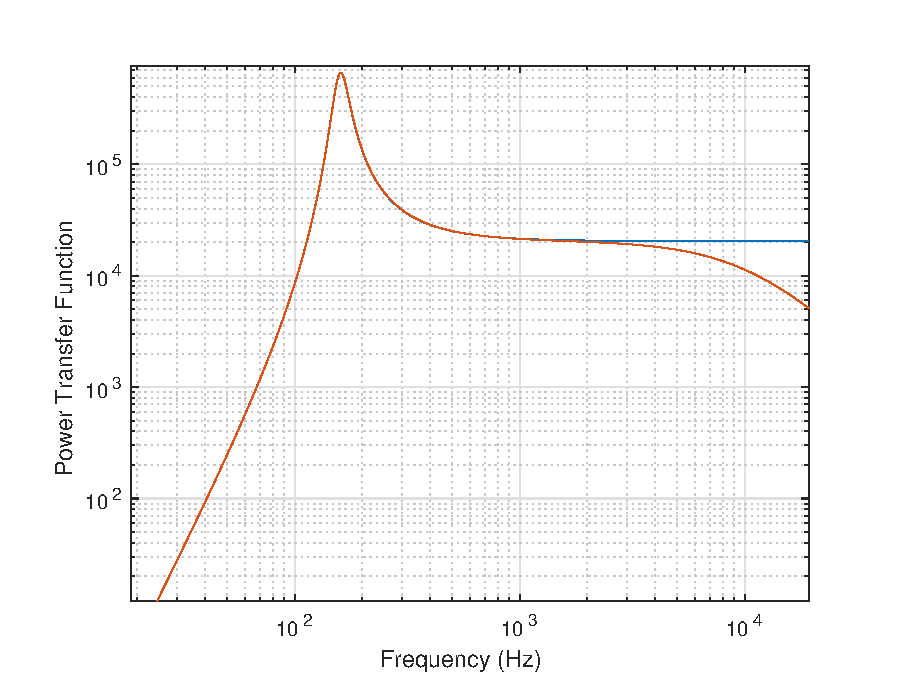
\includegraphics[width=.75\textwidth]{matlab/infiniteBafflePower.eps}
\caption{Infinite Baffle Power Transfer Function for $R_e=7$.
$C_{es}=1e-3$, $L_{es}=1e-3$, $R_{es}=30$. Red curve:$L_e=1e-4$, Blue curve: $L_e=0$}\label{fig:power-transfer}
\end{figure}

Looking into the power transfer function:
\begin{align}
G(\omega)=\left| \hat{H}(\omega)\right|^2 =\left| \frac{\omega  \hat{Z}_e }{ R_e+\hat{Z}_e} \right|^2\\
\hat{H}(\omega) =\frac{i L_{es}}{R_e}\frac{\omega^2}{-\omega^2 C_{es}L_{es}+i\omega L_{es}\left( R_e^{-1}+R_{es}^{-1} \right) +1}
\end{align}

We can recognize $\omega_s=\frac{1}{\sqrt{C_{es} L_{es}}}$ so we set the characteristic frequency $\omega_c=\omega_s$, and for clarity define $R_t=\frac{R_eR_{es}}{R_e+R_{es}}$:
\begin{align}
\hat{H}(\omega) =\frac{i }{R_eC_{es}}\frac{(\omega/\omega_c)^2}{-\frac{\omega^2}{\omega_c^2} +\frac{i \omega}{\omega_c}\frac{1}{R_t}\sqrt{\frac{ L_{es}}{C_{es}}} +1}\label{eq:freeair-transfer}
\end{align}
And, in the great reveal, we examine Equation \ref{eq:Qts} to find $Q_{ts}$ in terms of $R_{e}$, $R_{es}$, $L_{es}$, and $C_{es}$:
\begin{align}
Q_{ts}=\frac{R_e R_{es}}{R_e+R_{es}}\sqrt{\frac{C_{es}}{L_{es}}}\\
\hat{H}(\omega) =\frac{i \omega_s}{Q_{es}}\frac{(\omega/\omega_c)^2}{-\frac{\omega^2}{\omega_c^2} +\frac{i \omega}{\omega_c}\frac{1}{Q_{ts}}+1}
\end{align}

Which is the form of a second-order high-pass filter! Can we use this to turn the system in to a Butterworth filter with a flat pass-band and phase response? For a second order Butterworth filter:
\begin{align}
G(\omega)=\frac{(\omega/\omega_c)^4}{1+\left( \frac{\omega}{\omega_c} \right)^4}=\left| \frac{(\omega/\omega_c)^2}{-\left(\frac{\omega}{\omega_c} \right)^2 +\sqrt{2}\frac{i\omega}{\omega_c} +1} \right|^2
\end{align}
So if we can get $Q_{ts}^{-1}=\frac{ L_{es}}{R_{t}\sqrt{C_{es}L_{es}}} =\sqrt{2}$, our speaker will have a flat pass band and phase response! How can we do that? Well, if you put the back of the speaker in a sealed and enclosed area, there will be a $L_{ceb}$ in parallel to $L_{es}$ from the compliance (``springy-ness") of the air in the box -- we can use that to make our Butterworth filter by choosing the correct box volume!

\section{Sealed Box Enclosure} We're now able to attempt optimizing our sealed box replacing $L_{es}\rightarrow L_t=\left(L_{es}^{-1}+L_{ceb}^{-1}\right)^{-1}$ in Equation \ref{eq:freeair-transfer} and set it to the 2nd order Butterworth condition:
\begin{align}
\frac{ 1}{R_{t}}\sqrt{\frac{L_t}{C_{es}} } =\sqrt{2}\\
L_t=2R_{t}^2C_{es}\\
\frac{L_{es}L_{ceb}}{L_{es}+L_{ceb}}=2R_{t}^2C_{es}\\
L_{ceb}=\frac{2R_{t}^2C_{es}L_{es}}{L_{es}-2R_{t}^2C_{es}}\\
V_b=\frac{\rho c^2 S_d^2}{(B\ell)^2}\frac{2R_{t}^2C_{es}L_{es}}{L_{es}-2R_{t}^2C_{es}}
\end{align}

A perhaps more clear expression is:
\begin{align}
\frac{1}{L_{ceb}}=\frac{1}{2R_{t}^2C_{es}}-\frac{1}{L_{es}}
\end{align}

$L_{es}$ is commonly given in acoustic units of:
\begin{align}
V_{as}&=\rho c^2 S_d^2 L_{es}/(B\ell)^2\\
&=\rho c^2 S_d^2 L_{ms}
\end{align}
Converting the remaining terms to acoustic units yields:
\begin{align}
\frac{\rho c^2 S_d^2}{V_{b} (B\ell)^2}=\frac{1}{2C_{ms}Q_{ts}^2(B\ell)^2}
-\frac{\rho c^2 S_d^2}{V_{as} (B\ell)^2}\\
\frac{\rho c^2 S_d^2}{V_{b}}=\frac{\rho c^2 S_d^2}{2V_{as}Q_{ts}^2}
-\frac{\rho c^2 S_d^2}{V_{as}}\\
\frac{1}{V_{b}}=\frac{1}{2V_{as}Q_{ts}^2}
-\frac{1}{V_{as}}\\
V_{b}=V_{as}\frac{2Q_{ts}^2}{1-2Q_{ts}^2}
\end{align}
And generally, you can see the number 2 comes from $1/Q_t^2$ where $Q_t$ is the desired total system $Q$, therefore
\begin{align}
V_{b}=V_{as}\frac{(Q_{ts}/Q_{t})^2}{1-(Q_{ts}/Q_{t})^2}
\end{align}
Which is commonly described as the \textit{compression ratio} ($\alpha$):
\begin{align}
\alpha=\frac{V_{as}}{V_b}=\frac{1-(Q_{ts}/Q_{t})^2}{(Q_{ts}/Q_{t})^2}
\end{align}

That's it! Some important notes: sealed boxes only work if the current $Q_{ts}$ is less than the desired $Q_t$ (i.e., $Q_{ts}<Q_{t}$). For a 2nd order Butterworth filter, $Q_t\approx 0.7$, so $Q_{ts}>0.7$ to achieve B2 alignment. Also, it is possible to use other 2nd order filters to obtain specific design criteria by choosing a desired that is not B2 alignment. If $Q_{t}\neq 1/\sqrt{2}$, one can tune  low-frequency response and peak at $\omega_s$). The effect of choice of $Q$ is depicted in Figure \ref{fig:sealedBoxQ}.

\begin{figure}
\centering
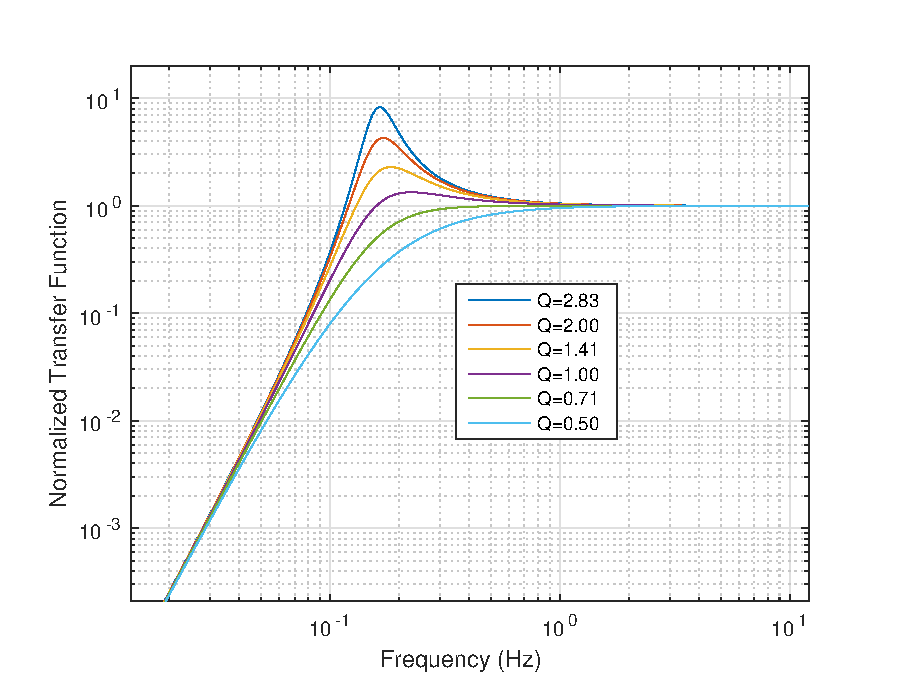
\includegraphics[width=0.75\textwidth]{matlab/sealedBoxQ.eps}
\caption{Normalized Acoustic Power in a Sealed Box Versus $Q$}\label{fig:sealedBoxQ}
\end{figure}

In this example, we only touched $L$, but it is also possible to similarly affect $R_t$ by adding an additional electric resistance in parallel with (or acoustic resistance in series with) the box compliance. That is the equivalent of filling the box with an acoustically absorbing material. This does two things: it properly adds compliance while keeping the speaker compact and it does not negatively effect efficiency, as seen in the previous discussion.

System resonance and roll-off frequency $f_3$ (corresponding to where response is $1/2$ of the peak value, or -3 dB, which describes the minimum frequency output of the system) will be changed. The new characteristic frequency $\omega_c$ and $f_3$ can be found with the addition of box compliance $C_{mb}$:
\begin{align}
\omega_c=\left( \sqrt{\frac{C_{ms}C_{mb}}{C_{ms}+C_{mb}}M_{ms}}  \right)^{-1}=\omega_s\sqrt{\frac{C_{ms}}{C_{mb}}+1}=\omega_s\sqrt{\frac{V_{as}}{V_{b}}+1}
\end{align}
and to find $\omega_3$:
\begin{align}
G(\omega_3)=1/2\\
\frac{(\omega_3/\omega_c )^4}{
\left[ -\left( \frac{\omega_3}{\omega_c} \right)^2 +\frac{1}{Q_t}\frac{i\omega_3}{\omega_c}+1\right]^{2}} = \frac{1}{2}\\
\left( \frac{\omega_3}{\omega_c} \right)^4 +\left( 2 -\frac{1}{Q_t^2}\right)\left(\frac{\omega_3}{\omega_c} \right)^2-1=0\\
\omega_3=\omega_c \left[ \frac{  \frac{1}{Q_{t}^2}-2  \pm \sqrt{\left( 2- \frac{1}{Q_{t}^2}\right)^2+4}}{2}\right]^{1/2}
\end{align}
Absolute values and $\pm$ is from finding the roots of a polynomial of order $w_3^4$, and allows for both peaked and low-pass responses.



Therefore, for a B2 closed-box alignment:
\begin{align}
\alpha&=\frac{1-2 Q_{ts}^2}{2 Q_{ts}^2} & \omega_3=\omega_c=\omega_s\sqrt{\alpha+1}
\end{align}

Finally, actual box dimensions can be chosen now that we know $V_b$. The most important thing is to choose irrational numbers to prevent standing waves. For example, the golden ratio ($0.6:1:1.6$) or ${2}^{-1/2}:{2}^{0}:{2}^{1/2}$ are sometimes used.

\section{Vented/Ported/Bass-Reflex Enclosures} Similar to the sealed box case, we can find the output power of a vented enclosure as seen in Figure \ref{bass_reflex} and \ref{fig:elec-mech-acoustic_model-simple}. Acoustic output is from the sum of two volume velocities corresponding to front and back radiation ($Q_f$ and $Q_b$). The total volume velocity is thus $Q_f-Q_b$, which in electrical units corresponds to  $v_s-v_{C_{Lev}}$. In electrical units, the acoustic output power can be calculated as:

\begin{align}
\begin{split}
\left\langle P_{ao} \right\rangle &=\frac{\left| v_s -v_{C_{lev}} \right|^2}{2R_{er}}=\frac{\left| v_{L_{cev}} \right|^2}{2R_{er}}=\frac{S_d^2 \rho\left| \omega \, v_{L_{cev}} \right|^2}{4\pi c (B \ell)^2}\\
&=\frac{S_d^2 \rho}{4\pi c (B \ell)^2}\left| \hat{H}_\omega \right|^2
\end{split}
\end{align}
and represents the fact that the front and back mechanical motions are $180^\circ$ out of phase.


%\begin{verbatim}
%Ze:(1/Rs+%i*\omega*Cs+1/(%i*\omega*Ls)
%    +1/(%i*\omega *Lb +1/(%i*\omega*Cv)) )^-1;
%full:(Ze/(Re+Ze))*(%i*\omega *Lb)/
%    (%i*\omega *Lb+1/(%i*\omega*Cv));
%factor((declare(\omega,mainvar),full));
%\end{verbatim}

\begin{align}
\hat{H}_\omega=\omega \, v_{L_{cev}}= \frac{
-i  C_{ev} L_{ceb} R_{es} L_{es} \omega^4}
{A'_4\omega^4-iA'_3\omega^3-A'_2\omega^2+iA'_1\omega+A'_0}\\
A'_4=C_{lev} L_{ceb} R_e R_{es}  C_{es} L_{es}\\
A'_3=C_{lev} L_{ceb} R_{es} L_{es}
+ C_{lev} L_{ceb} R_e L_{es}\\
A'_2=R_e R_{es}  C_{es} L_{es}+C_{lev} R_e R_{es} L_{es}+C_v L_{ceb} R_e R_{es}\\
A'_1=R_{es} L_{es}+R_e L_{es}\\
A'_0=R_e R_{es}
\end{align}
normalizing by $A'_0$ and defining $R_t=\frac{R_eR_{es}}{R_{es}+R_e}$, $Q_{t}=R_t\sqrt{\frac{C_{es}}{L_{es}}}$, $\omega_s=\frac{1}{\sqrt{C_{es}L_{es}}}$, and $\omega_b=\frac{1}{\sqrt{C_{lev}L_{ceb}}}$
\begin{align}
\hat{H}(\omega)=\omega \, v_{L_{cev}}= \frac{
-i  C_{ev} L_{ceb} L_{es} \omega^4/R_e}
{A_4\omega^4-iA_3\omega^3-A_2\omega^2+iA_1\omega+1}\\
\hat{H}(\omega)= \frac{-i\omega_s}{Q_{es}}\frac{\omega^4/\omega_b^2 \omega_s^2}
{A_4\omega^4-iA_3\omega^3-A_2\omega^2+iA_1\omega+1}\\
A_4=C_{lev} L_{ceb} C_{es} L_{es}=\frac{1}{\omega_b^2\omega_s^2}\\
A_3=\frac{C_{lev} L_{ceb} L_{es}}{R_t}=\frac{1}{\omega_b^2\omega_s Q_{t}}\\
A_2=C_{es} L_{es}+C_{lev} L_{es}+C_{lev} L_{ceb}=\frac{1}{\omega_s^2}+\frac{1}{\omega_b^2}+\frac{L_{es}}{L_{eb}}\frac{1}{\omega_b^2}\\
A_1=\frac{L_{es}}{R_t}=\frac{1}{Q_{t}\omega_s}
\end{align}

%\begin{verbatim}
%Ze:(1/Rs+%i*\omega*Cs+1/(%i*\omega*Ls)
%    +1/(%i*\omega *Lb +1/(%i*\omega*Cv)) )^-1;
%full:(Ze/(Re+Ze))*(%i*\omega *Lb)/
%    (%i*\omega *Lb+1/(%i*\omega*Cv));
%factor((declare(\omega,mainvar),full));
%\end{verbatim}

This can be seen as a 4th order filter, we just have to choose our the variables to properly ``align" with the audio response we want. Thiele observed that for drivers with $Q_t=0.383$, a ``perfect" fourth order Butterworth filter can be made if $\omega_b$ and $V_b$ are chosen properly; when $Q_t<0.383$, you can get a ``Quasi-Butterworth Third Order" alignment; and for drivers $Q_t>0.383$ a ``Fourth Order Chebyschev" alignment is suitable. Both Thiele and Small created tables and graphical tools to aid design. Modern computers give us an alternative tool which is especially helpful for two- or three-way speakers (multiple drivers in the same box). For completeness, we will find the analytical expressions then describe how computers can be used.

\subsection{Fourth Order Butterworth Filter (B4) \texorpdfstring{\\$Q_t=0.383$}{Qt=0.383}} A fourth order Butterworth filter produces a power response of the form:
\begin{align}
\left|  \hat{H}(\omega) \right|^2&\propto \frac{(\omega/\omega_c)^8}{1+\left(\frac{\omega}{\omega_c}\right)^8}\label{eq:transfer_func}\\
\begin{split}
\hat{H}(\omega)&=\frac{(\frac{\omega}{\omega_c})^4}{(\frac{\omega}{\omega_c})^4-i2.6132(\frac{\omega}{\omega_c})^3-3.414(\frac{\omega}{\omega_c})^2+i2.613(\frac{\omega}{\omega_c})+1}\\
&=\frac{(\frac{\omega}{\omega_c})^4}{(\frac{\omega}{\omega_c})^4-iA_3(\frac{\omega}{\omega_c})^3-A_2(\frac{\omega}{\omega_c})^2+iA_1(\frac{\omega}{\omega_c})+1}
\end{split}
\end{align}

We can now use this to design the box by using Equation \ref{eq:transfer_func} to generate the following relationships:
\begin{align}
\omega_c&=\sqrt{\omega_b \omega_s}=\omega_3\\
A_1/\omega_c&=1/Q_t\omega_s\\
A_2/\omega_c^2&=1/\omega_s^2+1\omega_b^2+(L_{es}/L_{eb})(1/\omega_b^2)\\
A_3/\omega_c^3&=1/\omega_b^2\omega_sQ_t
\end{align}
where $\omega_c$ is the characteristic frequency of the box, which in the case of the B4 filter is also the frequency where Equation \ref{eq:transfer_func} is $1/2$ of the maximum value (i.e., 3dB lower, $\omega_3$). This gives us our dimensions for the box!

\begin{align}
\frac{V_{as}}{V_{b}}&=\frac{A_1A_2A_3-A_1^2-A_3^2}{A_3^2}=\alpha\label{eq:dimensions-start}\\
\frac{\omega_b}{\omega_s}&=\frac{A_1}{A_3}=h\\
\omega_b&=(C_{ev}L_{eb})^{-1}=\frac{c^2A_v}{V_bl_v}=h\omega_s\\
\frac{l_v}{A_v}&=\frac{\alpha c^2}{V_{as} h \omega_s}\\
Q_t&=\frac{1}{\sqrt{A_1A_3}}\label{eq:dimensions-end}
\end{align}

For a B4 alignment, yields:
\begin{align}
\omega_c=\omega_s=\omega_b\\
Q_t=0.383\\
\frac{L_{es}}{L_{eb}}=\frac{V_{as}}{V_{ab}}=1.414
\end{align}
which allows us to write $\hat{H}(\omega)$ as:
\begin{align}
\hat{H}(\omega)=\frac{\left(\frac{-i\omega_c}{Q_{es}}\right)\left(\frac{\omega}{\omega_c}\right)^4}
{\left(\frac{\omega}{\omega_c}\right)^4-i\frac{1}{Q_t}\left(\frac{\omega}{\omega_c}\right)^3-\left(2+\frac{L_{es}}{L_{eb}}\right)\left(\frac{\omega}{\omega_c}\right)^2+i\frac{1}{Q_t}\frac{\omega}{\omega_c}+1}
\end{align}

To make a forth order Butterworth box:
\begin{enumerate}
\item Make the box volume is: $V_b=\frac{1}{\sqrt{2}}V_{as}$
\item The vent dimensions are: $\frac{A_v}{l_v}=\frac{\omega_s^2 V_{as}}{c^2\sqrt{2}}$. This is found from $\omega_b^2=\omega_s^2=\frac{1}{C_{ev}L_{eb}}=\frac{1}{V_b l_v/(c^2 A_v)}=\frac{\sqrt{2}c^2 A_v}{V_{as}l_v}$
\item $Q_t$ will need to be tuned by placing a resistor in series with the speaker, thus effectively increasing $R_e$. Therefore, in this alignment (i.e., this choice of filter parameters), only $Q_{ts}>0.383$ are easily implemented. However, this technique of using a resistor to decrease $Q_{es}$ is rarely\footnote{rarely=never} done since it also reduces output power when similar performance can be found with the Chebyschev (C4) alignment described below.
\end{enumerate}

The fourth order Butterworth (i.e., ``B4") filter only really is suitable for $Q_t=0.383$ drivers. Other alignments make vented boxes for other $Q_t$ possible.

\subsection{Fourth Order Chebyschev (C4) \texorpdfstring{\\$Q_t>0.383$}{Qt>0.383}}
Thiele uses the fact that Chebyschev filters are Butterworth filters where the real part of the Butterworth filter poles (i.e., the roots of the denominator) are multiplied by the same factor $k$. For example, in a B4 filter (with $s=i\omega/\omega_c$), the poles are the roots of the denominator of the low-pass transfer function:
\begin{align}
\hat{H}(s)=\frac{1}{
s^4+2.6132s^3+3.414s^2+2.613s+1}\\
s=\{-0.3827\pm 0.9239i;-0.9239 \pm 0.3827i\}\label{eq:cheby_roots}
\end{align}
We can therefore convert the B4 filter to a Chebyshev filter form by multiplying the real part of each of the roots by $k$ which gives us a low-pass Chebyshev filter of the form:
\begin{align}
\hat{H}(s)= \prod_i \frac{-1}{ s/p_i-1 }= \prod_i  \frac{-p_i}{ s-p_i }
\end{align}
where $i$ is the index of the $i$th pole.

The low-pass Chebyshev filter that has the same roots described in Equation \ref{eq:cheby_roots} is:
\begin{align}
\hat{H}(s)=\frac{a_4}{s^4+a_1s^3+a_2s^2+a_3s+a_4}\label{eq:cheby_low}
\end{align}
where:
\begin{align}
\begin{split}
a_1&=2.6131k \\
a_2&=2.4143k^2+1\\
a_3&=0.9239k^3+1.6892k \\
a_4&=0.1250k^4+0.7500k^2+0.1250\\
\end{split}
\end{align}
Transforming Equation \ref{eq:cheby_low} to a high-pass filter means changing all $s\rightarrow s^{-1}$:
\begin{align}
\hat{H}(s)=\frac{a_4s^4}{1+a_1s+a_2s^2+a_3s^3+a_4s^4}
\end{align}
The frequency response ($s=i\omega/\omega_c$) is therefore:
\begin{align}
\hat{H}(s)=\frac{a_4\left(\frac{\omega}{\omega_c}\right)^4}{1+i a_1\left(\frac{\omega}{\omega_c}\right)-a_2\left(\frac{\omega}{\omega_c}\right)^2-ia_3\left(\frac{\omega}{\omega_c}\right)^3+a_4\left(\frac{\omega}{\omega_c}\right)^4}
\end{align}
and defining a new $\omega'_c=\omega_c /a_4^{1/4}$:
\begin{align}
\hat{H}(s)&=\frac{\left(\frac{\omega}{\omega'_c}\right)^4}{1+i\frac{a_1}{a_4{1/4}}\left(\frac{\omega}{\omega'_c}\right)-\frac{a_2}{a_4{1/2}}\left(\frac{\omega}{\omega'_c}\right)^2-i\frac{a_3}{a_4{3/4}}\left(\frac{\omega}{\omega'_c}\right)^3+\left(\frac{\omega}{\omega'_c}\right)^4}\\
&=\frac{\left(\frac{\omega}{\omega'_c}\right)^4}{1+iA_1 \left(\frac{\omega}{\omega'_c}\right)-A_2\left(\frac{\omega}{\omega'_c}\right)^2-iA_3\left(\frac{\omega}{\omega'_c}\right)^3+\left(\frac{\omega}{\omega'_c}\right)^4}\label{eq:c4-transfer}
\end{align}
where:
\begin{align}
\omega_c'&=\sqrt{\omega_b\omega_s}\\
A_1&=\frac{2.6131k}{(0.1250k^4+0.7500k^2+0.1250)^{1/4}} \\
A_2&=\frac{2.4143k^2+1}{(0.1250k^4+0.7500k^2+0.1250)^{2/4}} \\
A_3&=\frac{0.9239k^3+1.6892k}{(0.1250k^4+0.7500k^2+0.1250)^{3/4}}
\end{align}
When $k=1$, you can see that the $A_1$, $A_2$, $A_3$ are the same as the B4 coefficient alignments when $k=1$.

We can now find the dimensions and performance specifications for our speaker! First we need to find what $k$ corresponds to our speaker. This can be found from our driver's specified $Q_t$ and solving for $k$:
\begin{align}
Q_t=\frac{1}{\sqrt{A_1A_3}}
\end{align}
Next we find the volume of the box from $V_{as}/V_{b}=L_{es}/L_{eb}$:
\begin{align}
\frac{V_{as}}{V_{b}}=\frac{A_1A_2A_3-A_1^2-A_3^2}{A_3^2}=\alpha
\end{align}
We find the required $\omega_b$ (i.e., the dimensions of the port as a function of box volume) from:
\begin{align}
\frac{\omega_b}{\omega_s}&=\frac{A_1}{A_3}=h
\end{align}
and the characteristic frequency frequency from:
\begin{align}
\omega_c'&=\sqrt{\omega_b\omega_s}=\omega_s\sqrt{h}
\end{align}
Finally, the cut-off frequency (when 3dB lower than the value at high frequencies) is given by solving for when the power spectrum (i.e., the square of the magnitude of Equation \ref{eq:c4-transfer}) is $1/2$ of the high-frequency value.

\begin{align}
\hat{H}(\omega)&=\frac{\left(\frac{\omega}{\omega'_c}\right)^4}{1+iA_1 \left(\frac{\omega}{\omega'_c}\right)-A_2\left(\frac{\omega}{\omega'_c}\right)^2-iA_3\left(\frac{\omega}{\omega'_c}\right)^3+\left(\frac{\omega}{\omega'_c}\right)^4}\\
\left| \hat{H}(\omega_3) \right|^2 &=\frac{\left(\frac{\omega_3}{\omega'_c}\right)^8}{1+B_1 \left(\frac{\omega_3}{\omega'_c}\right)^2+B_2\left(\frac{\omega_3}{\omega'_c}\right)^4+B_3\left(\frac{\omega_3}{\omega'_c}\right)^6+\left(\frac{\omega_3}{\omega'_c}\right)^8}=\frac{1}{2}\\
B_1 &= A_1^2-2A_2\\
B_2 &= 2+A_2^2-2A_1A_3\\
B_3 &= A_3^2-2A_2
\end{align}

So to find $\omega_3$ you fist need to find the roots of:
\begin{align}
\frac{1}{\left(\frac{\omega'_c}{\omega_3}\right)^8+B_1 \left(\frac{\omega'_c}{\omega_3}\right)^6+B_2\left(\frac{\omega'_c}{\omega_3}\right)^4+B_3\left(\frac{\omega'_c}{\omega_3}\right)^2+1}&=\frac{1}{2}\\
\left(\frac{\omega'_c}{\omega_3}\right)^8+B_1 \left(\frac{\omega'_c}{\omega_3}\right)^6+B_2\left(\frac{\omega'_c}{\omega_3}\right)^4+B_3\left(\frac{\omega'_c}{\omega_3}\right)^2-1&=0\\
d^4-B_3 d^3- B_2 d^2 - B_1 d -1&=0
\end{align}
where $d=(\omega_3/\omega_c')^2$. Taking the largest real root of $d$ yields:
\begin{align}
\frac{\omega_3}{\omega_s}=\sqrt{dh}
\end{align}

\subsection{Third Order Quasi-Butterworth (QB3) \texorpdfstring{\\$Q_t<0.383$}{Qt<0.383}} When $Q_t<0.38$, you can use a ``Third Order Quasi-Butterworth" alignment. This filter is described by the transfer function:
\begin{align}
\left| \hat{H}(s) \right|^2 &=\frac{(\omega/\omega_c)^8}{(\omega/\omega_c)^8+B^2(\omega/\omega_c)^2+1}
\end{align}
Which reduces to a fourth order Butterworth filter $B=0$. We can see what generic filter behaves like this QB3 filter by comparing a generic fourth-order filter with the form:
\begin{align}
\hat{H}(\omega) &=\frac{(\omega/\omega_c)^4}{(\omega/\omega_c)^4-iA_3(\omega/\omega_c)^3-A_2(\omega/\omega_c)^2+iA_1(\omega/\omega_c)+1}
\end{align}
therefore, to be a QB3 filter:
\begin{align}
A_3^2-2 A_2&=0\label{eq:qb3-start}\\
2+A_2^2-2 A_1 A_3&=0\\
A_1^2-2 A_2&=B^2\label{eq:qb3-end}
\end{align}
therefore:
\begin{align}
A_3&=\sqrt{2 A_2}\\
A_1&=\frac{2+A_2^2}{2 A_3}=\frac{2+A_2^2}{2 \sqrt{2 A_2}}
\end{align}

Using equations \ref{eq:dimensions-start}--\ref{eq:dimensions-end} with \ref{eq:qb3-start}--\ref{eq:qb3-end} yields:
\begin{align}
\frac{w_b}{w_s}&= \frac{1}{Q_t\sqrt{8-8Q_t^2}}=h\\
\omega_c&=\sqrt{\omega_s \omega_b}\\
A_2&=\frac{1}{2 Q_t^2 h}=\sqrt{2(1/Q_t^2-1)}\label{eq:qb3-power}
\end{align}
from which $A_1$, $A_3$, and $B$ can be calculated, and which will give us the box dimensions.

We also can model the box's performance. The low frequency cut-off $\omega_3$ (i.e., 3 dB down from the high-frequency response) can be found from making Equation \ref{eq:qb3-power} equal $1/2$ and solving for $\omega/\omega_c$. Then using the relationship that $\omega_3\sqrt{h}/\omega_c=\omega_3/\omega_s$, we can find the normalized cut-off frequency:
\begin{align}
\frac{1}{1+B^2\left( \frac{\omega_c}{\omega_3} \right)^6+\left( \frac{\omega_c}{\omega_3} \right)^8}=\frac{1}{2}\\
\left( \frac{\omega_3}{\omega_c} \right)^8-B^2\left( \frac{\omega_3}{\omega_c} \right)^2-1=0\\
\frac{\omega_3}{\omega_s}=\sqrt{h}\frac{\omega_3}{\omega_c}
\end{align}

\section{Graphical Tool for Enclosure Design} Small's paper used the equations for CB4 and QB3 filters to generate plots where one can find the compresion ratio $\alpha=V_{as}/V_{b}$, box frequency $h=\omega_b/\omega_s$, speaker $Q_t$, and cut-off frequency $\omega_3/\omega_s$ if one of those variables were known. Using the code from Appendix \ref{appendix:qt-matlab}, we can generate such a figure as seen in Figure \ref{fig:qt-matlab}. If the proper parameters are chosen, the normalized power transfer function follows Figure \ref{fig:powertransfer-matlab}.


\begin{figure}
\centering
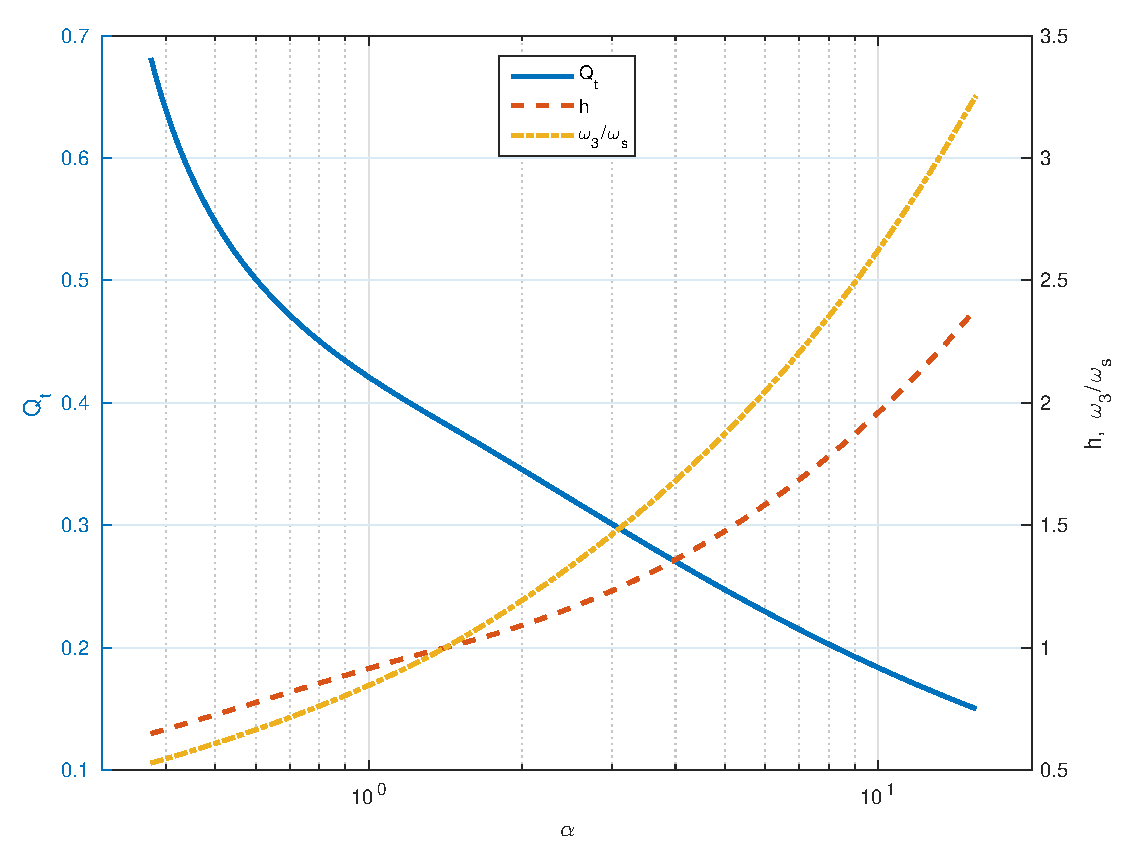
\includegraphics[width=0.75\textwidth]{matlab/vented_design.eps}
\caption{Graphical solution for finding compression ratio $\alpha$, normalized box and cut-off frequencies ($h$ and $\omega_3$) for a given $Q_t$}\label{fig:qt-matlab}
\end{figure}

\begin{figure}
\centering
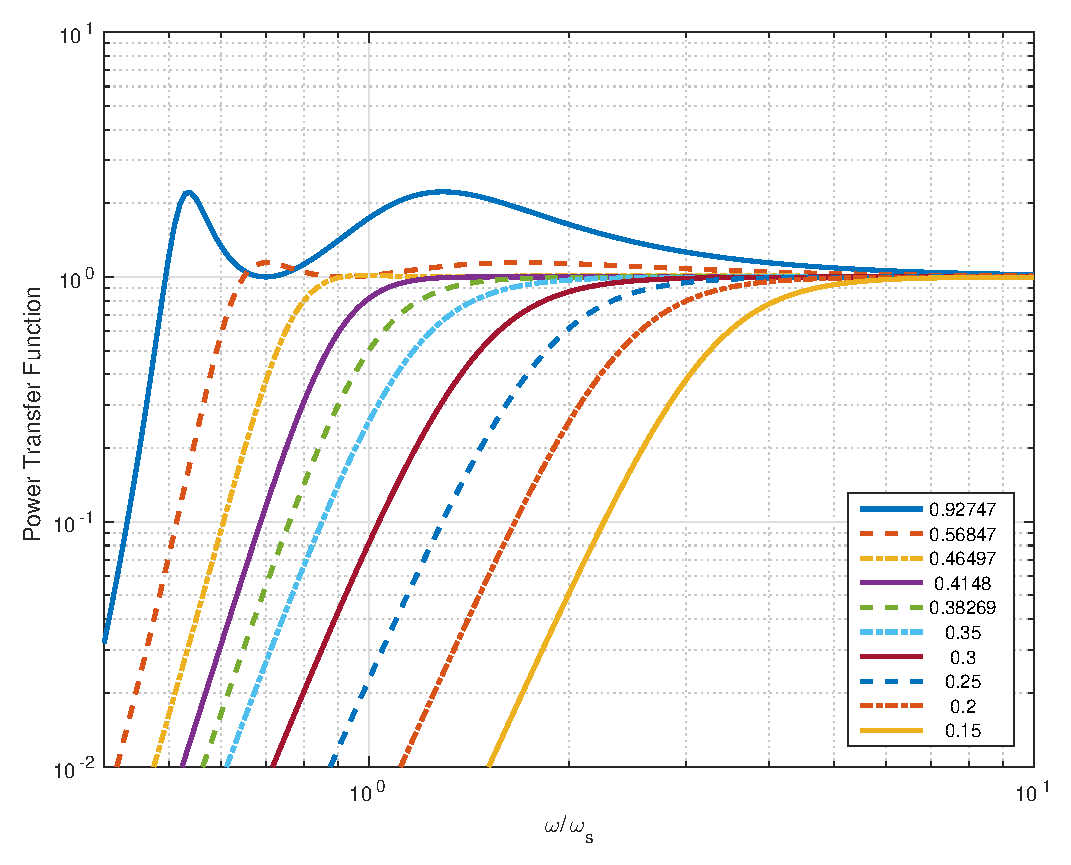
\includegraphics[width=0.75\textwidth]{matlab/chebyfilters.eps}
\caption{Power transfer function as function of $Q_t$}\label{fig:powertransfer-matlab}
\end{figure}

\subsection{Closed or Vented Box?}
The choice between the closed/sealed or vented/ported design is based on the available driver specifications and desired frequency response. For example, Figure \ref{fig:sealed_vs_ported_design} shows a comparison of performance and design values between a B2 closed box(thin lines) and a QB3-B4-C4 vented box (thick lines). Some conclusions can be drawn: (1) vented boxes always have a lower $\omega_3$ than closed boxes for a given $Q_t$ and (2) closed boxes are smaller than vented boxes when $Q_t<0.6$.



An additional too to aid decisions is to look at the \textit{efficiency bandwidth product} (EBP), defined by Richard Small\footnote{Commonly attributed to Small, but I have not been able to find the original citation} as:
\begin{align}
\mbox{EBP}=\frac{\omega_s}{2\pi Q_{es}}=\frac{f_s}{Q_{es}}
\end{align}

Prof. Small is attributed to have given the following guidelines to interpret EBP: a speaker with an EBP$>100$ is well suited for a ported design, EBP$<50$ is well suited for a closed design, and $50<$EBP$<100$ could be either. This can be seen as an interpretation of Figure \ref{fig:sealed_vs_ported_design}. If a speaker has high $f_s$, you want to use the ported design to get the lowest $\omega_c$. If a speaker has a high $Q_{es}$ and thus a high $Q_t$, $\omega_c$ will be already be low, so using the smaller sealed box can be convenient.



\begin{figure}
\centering
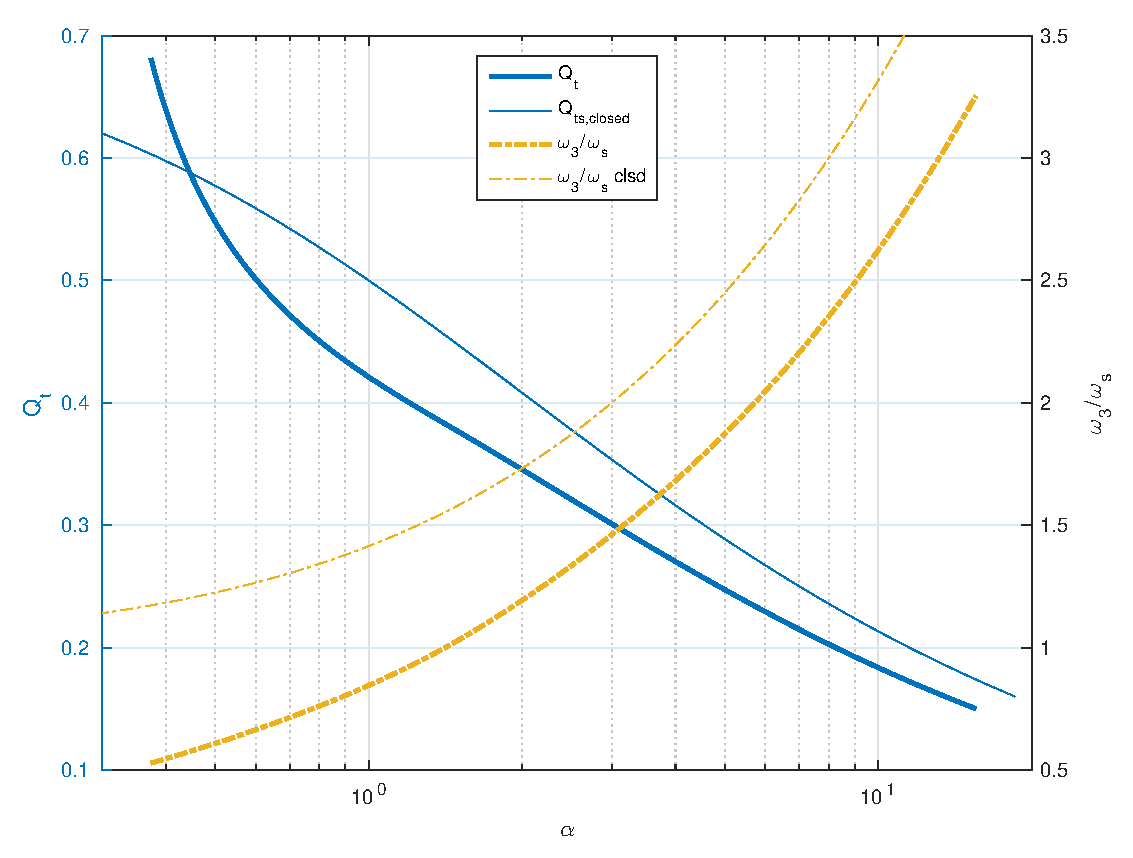
\includegraphics[width=.75\textwidth]{matlab/sealed_vs_ported_design.eps}
\caption{Relationship between compression ratio ($\alpha$), normalized cut-off frequencies ($\omega_3$) for a given $Q_t$ (vented box, thick lines); $\alpha$, $\omega_3/\omega_s$, and $Q_{ts}$ (closed box, thin lines)}\label{fig:sealed_vs_ported_design}
\end{figure}

\section{Group Delay?}

\section{Excursion and Power ratings?}

\section{Efficiency?}

\section{Including effects of loss?}

\section{Computer Design:} Given a user defined ``range of interest" of frequencies (e.g., 20 Hz-20 kHz), and driver specifications, minimize RMS error of SPL given a constraint of max box size. Simultaneously optimize for two speakers (similar efficiencies).



\subsection{Two-way Speaker Design}
Optimize box for low-frequency only, but impedance match features in pass bands?

http://www.audioholics.com/loudspeaker-design/

cross-over 2x above fs

inductor for woofer to protect it?

\textbf{efficiency}
Back to model - get rid of backwards waves with a big baffle, now we are delivering energy.

efficiency: simply $(v_rad^2/Rrad) / (vin^2/totalR)$

The goal is to delivery energy to the acoustic transmission, can we help impedance match? elements you need for impedance match = Helmholtz resonator! get vent 180 degrees out of phase for free! Get all electrical energy on to real part (both mechanical resistance and sound). Good = more efficient, bad=what if system has bad Q? too much energy(forces) on resistors/mechanical elements? impedance mismatch with Re Le?

well designed box, minimize electronic impedance matching!

Why sealed box? impedance match mass.


\hrule

efficiency is proportional to difference in voltage over res and voltage over rev (assuming vent losses are low). voltage is transferred to Q

\textbf{when there is no box, $Q_b=Q_l=0$, load is inductive and added to $M_ms$}

should i make inductors all value of M?


\textbf{$\mu$ for air is $1.56\times10^{-5}$m$^2$/s.}

\textbf{split variable definitions in to electrical mechanical acoustic Also derived variables?}

\textbf{EBP - compare efficiency of sealed to vented, when does one win?}

references:
\begin{verbatim}
Website:
andyc.diy-audio-engineering.org/vented_box_2.xhtml
\end{verbatim}
f3 is in small's appendices

\appendix

\chapter{random stuff}
time avg power
\begin{align}
\left\langle P_L \right\rangle&=\lim_{T\rightarrow \infty} \int_{t=0}^{t=T} VI\, dt\\
\left\langle P_L \right\rangle &=\lim_{T\rightarrow \infty} \int_{t=0}^{t=T} \Re\{\hat{v}_L e^{i\omega t}\}\Re \left\{ \frac{\hat{v}_L }{\hat{Z}_L}e^{i \omega t} \right\} \, dt\\
\left\langle P_L \right\rangle &=\int_{t=0}^{t=\frac{2\pi}{\omega}} \left| \hat{v}_L \right|
                                 \cos (\omega t+\phi_v)
                                \left(
                                  \frac{ \left| \hat{v}_L \right|}
                                    {\left| \hat{Z}_L \right| }
                                  \cos(\omega t +\phi_v - \phi_{\hat{Z}_L})
                                \right) \, dt\\
\left\langle P_L \right\rangle &= \frac{\left| \hat{v}_L \right|^2}{2\left| \hat{Z}_L\right|}\cos\phi_{\hat{Z}_L}=\left| \hat{v}_0 \right|^2\frac{\left| \hat{Z}_L\right|}{2\left| R_g+\hat{Z}_L\right|^2}\cos\phi_{\hat{Z}_L}\label{eq:time-avg-pwr-load}
\end{align}
where $\hat{Z}_L=\left| \hat{Z}_L \right| e^{i\phi_{\hat{Z}_L}}$.

\chapter{QB3, C4 Alignment Code}\label{appendix:qt-matlab}
%\lstinputlisting[language=Matlab]{matlab/vented_design.m}
 
\end{document}